\chapter{Sensores RGB-D}\label{sensores_rgbd}
El área de visión en computación es un área de investigación que está constantemente en desarrollo y la cual tiene cada vez más aplicaciones en problemas del mundo real. Durante los últimos años y con el poder de cómputo de los nuevos procesadores se ha posibilitado el desarrollo de nuevos y mejores algoritmos utilizando más información del entorno, manteniendo tiempos de ejecución razonables para aplicaciones de tiempo real.

Dentro de estos avances logrados en el área, los sensores RGB-D otorgan una novedosa forma de obtener datos visuales del ambiente. Estos sensores están conformados típicamente por una cámara tipo web común RGB que captura el mundo en dos dimensiones (2D), es decir, las texturas o colores del mundo real y por otra parte tienen una cámara de profundidad que provee información de la distancia de los distintos objetos de la escena a la cámara.

La cámara o sensor de profundidad consta de dos elementos: un proyector infrarrojo y una cámara infrarroja. Para poder medir la profundidad de todo lo presente en la escena el proyector imprime con luz infrarroja un patrón conocido. Esta luz es invisible al ojo humano y a las cámaras RGB convencionales. Sin embargo, sí se puede ver con una cámara infrarroja. La cámara infrarroja entonces, se utiliza para obtener el patrón dibujado en la escena. Conociendo el patrón original proyectado, el patrón obtenido con la cámara y la distancia entre la cámara infrarroja y el proyector se pueden aplicar algoritmos de luz estructurada para obtener la profundidad de la escena.

Existen varias implementaciones de cámaras que otorgan esta información y cada una tiene sus propias características en cuanto a calidad de la imagen RGB, frecuencia de cuadros, rango de profundidad, etc. La más conocida de estas cámaras es la llamada ``Kinect'' de Microsoft. Esta cámara posee una resolución default en RGB de unos 640x480 píxeles de 8 bits cada uno, a unos 30 cuadros por segundo. La misma puede otorgar imágenes de hasta 1280x1024 píxeles pero a una frecuencia de cuadros menor. En el caso del video en profundidad, el sensor provee una resolución de imagen de unos 640x480 píxeles y cada uno de ellos tiene una resolución de 11 bits, lo que da una sensibilidad de 2048 niveles. La frecuencia de cuadros que otorga el sensor de profundidad es de unos 30 cuadros por segundo. El rango práctico de distancias que ofrece la cámara está entre 1.2 y 3.5 m, aunque puede dar un rango extendido de unos 0.7 a 6 m. En la Figura \ref{fig:sensores_rgbd} se puede ver un esquema de los sensores más populares: ``Kinect'' de Microsoft y ``Xtion'' de Asus.

\begin{figure}
	\centering
	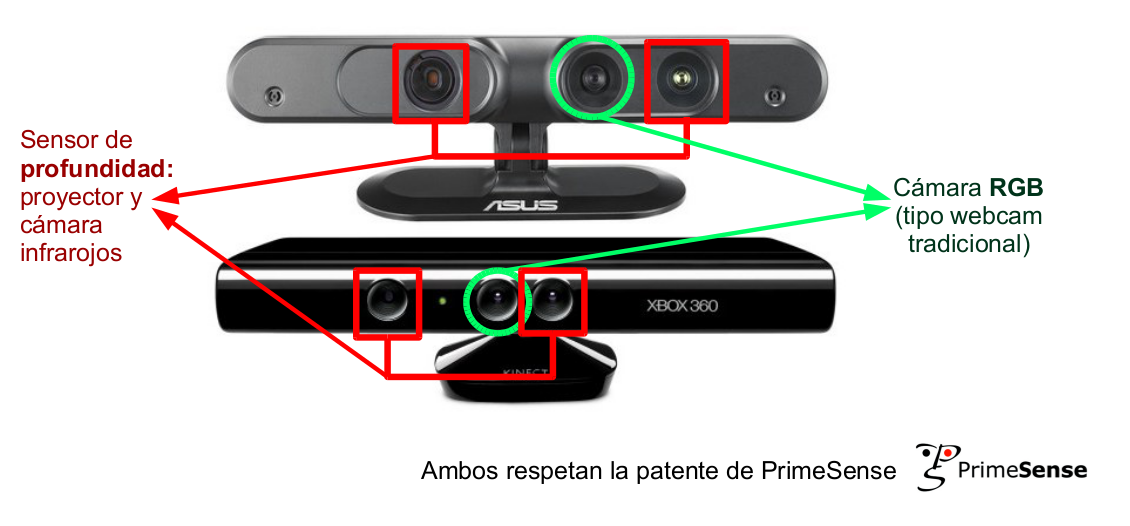
\includegraphics[width=\textwidth]{img/sensores/sensores_rgbd.png}
	\caption{Esquema de los sensores RGB-D. Arriba está el sensor Xtion de Asus. Abajo está el Kinect de Microsoft.}
    \label{fig:sensores_rgbd}
\end{figure}

Una de las características de los sensores de profundidad de este tipo es que al utilizar luz infrarroja no necesitan luz para funcionar y obtener información. De manera contraria a una cámara RGB, este sensor se ve perjudicado por la luz solar ya que el sol emite luz infrarroja que interfiere con el patrón dibujado por el proyector, haciendo que los datos obtenidos no sean correctos. Además el método se ve perjudicado cuando existen en la escena objetos como vidrios, espejos y superficies brillantes ya que los haces de luz son reflejados y por lo tanto se modifica el patrón proyectado por el sensor.

La información de profundidad puede utilizarse en conjunto con la de color para rearmar la escena en 3D. Conociendo los parámetros de calibración de la cámara se puede calcular en donde se ubica cada píxel dentro de una escena en 3D y de esta manera obtener lo que se llama ``nube de puntos''. Una nube de puntos es un conjunto de 3-uplas en donde cada valor corresponde a una distancia para cada uno de los ejes que representan un espacio 3D. En la Figura \ref{nube_de_puntos_sola} podemos ver un ejemplo de este tipo de nube de puntos. Cuando se combina una nube de puntos con la información 3D, se puede obtener una nube de puntos más completa, como las que se muestran en la Figura \ref{nube_de_puntos_color}.

\begin{figure}
	\centering
	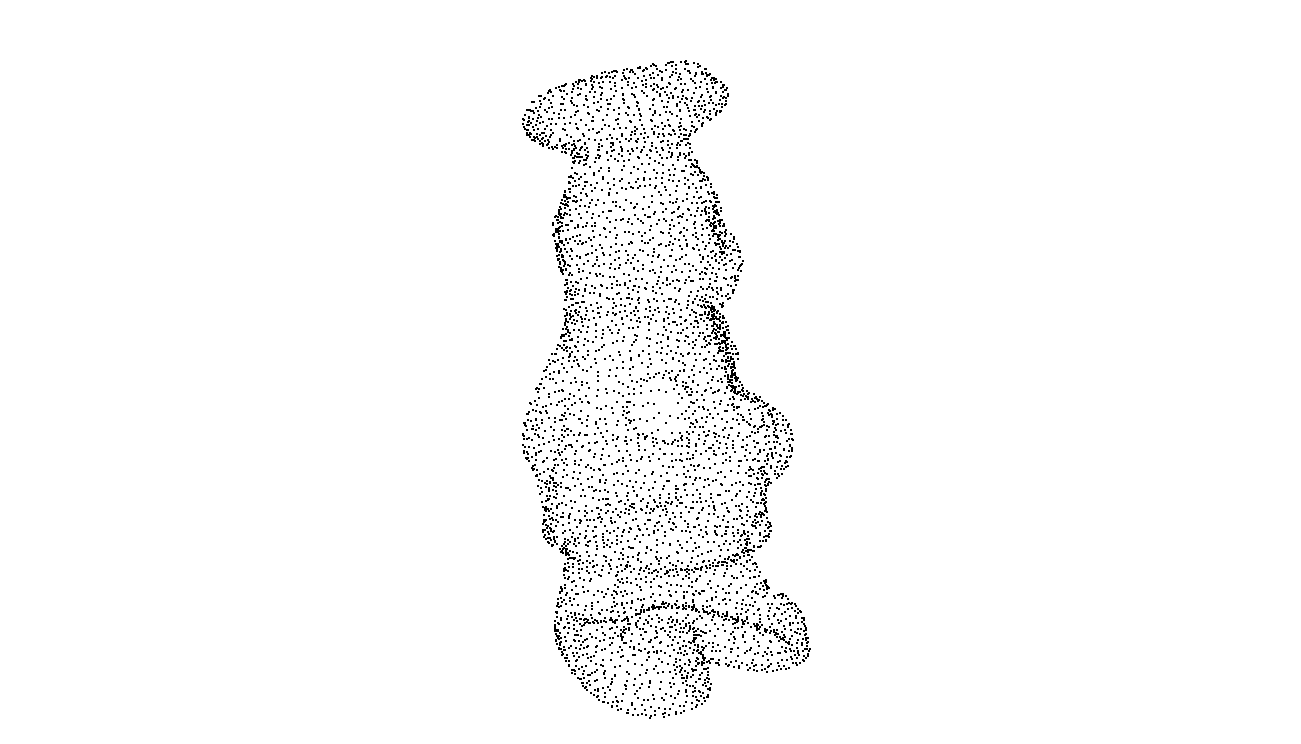
\includegraphics[width=\textwidth]{img/nube_de_puntos_sola.png}
	\caption{Nube de puntos}
    \label{nube_de_puntos_sola}
\end{figure}


\begin{figure}
	\centering
    \begin{subfigure}[b]{0.5\textwidth}
		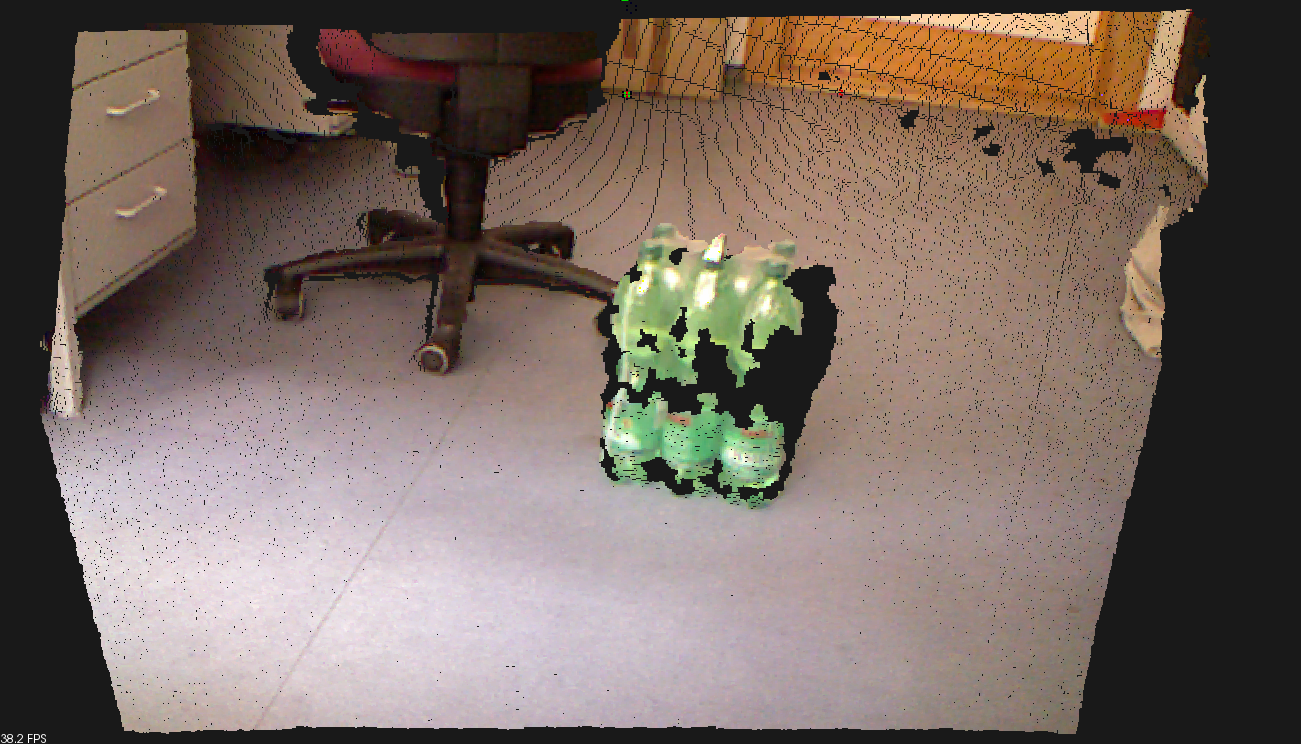
\includegraphics[width=\textwidth]{img/nube_de_puntos_color_1.png}
	\end{subfigure}
	\begin{subfigure}[b]{0.5\textwidth}
		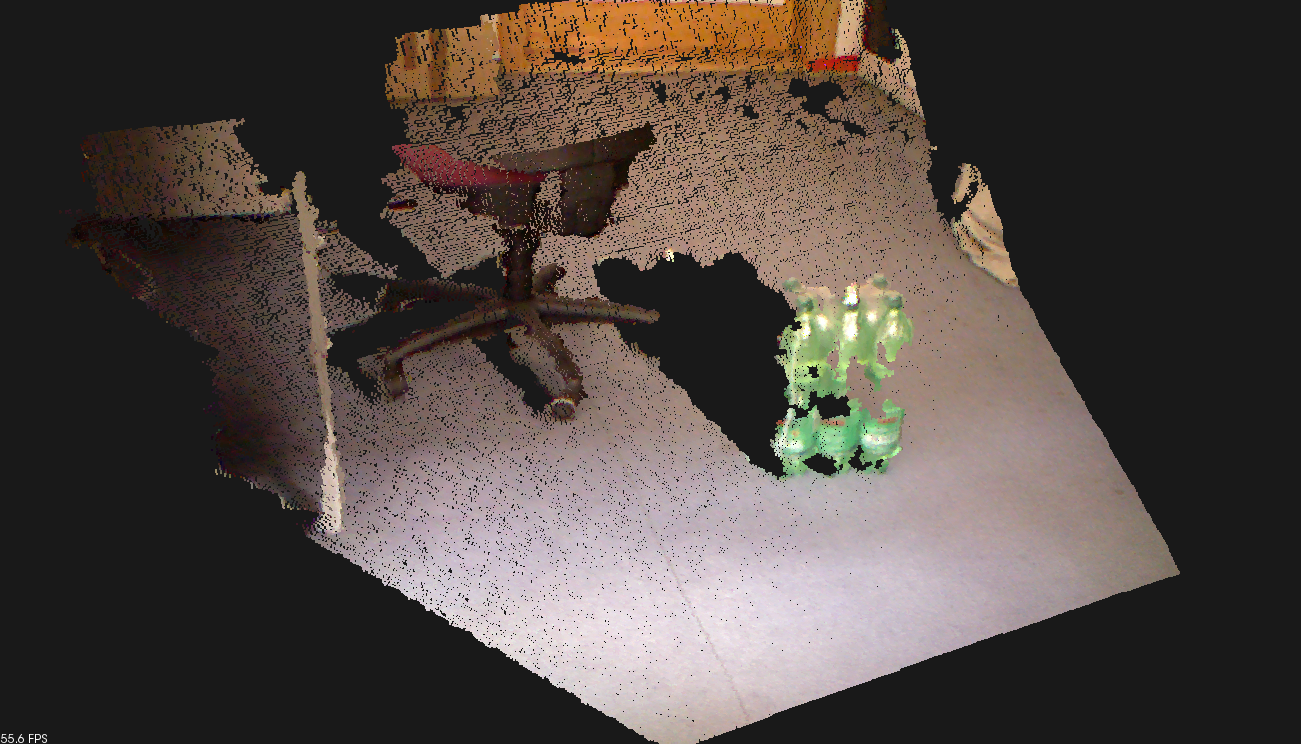
\includegraphics[width=\textwidth]{img/nube_de_puntos_color_2.png}
	\end{subfigure}
	\caption{Nube de puntos con información RGB vista desde dos ángulos distintos}
    \label{nube_de_puntos_color}
\end{figure}


La información provista por este tipo de imágenes no sólo complementa la información a color de una imagen RGB sino que abre la puerta a nuevas maneras de interactuar con el entorno. Con las imágenes RGB solo se puede capturar una parte del mundo como lo percibimos. Al no tener información de profundidad resulta difícil por ejemplo, lidiar con problemas de escala de los objetos o definir los bordes de un objeto con poca textura o cuyo color es similar al color de fondo. Con la información 3D las imágenes se asemejan más al mundo que percibimos los seres humanos.

Esta tecnología lleva un tiempo siendo explorada y existen distintas áreas en donde hacen uso de la misma. Un ejemplo de ello es la cámara nombrada previamente, ``Kinect''. Esta cámara comenzó a utilizarse en la consola de videojuegos ``XBox'' de \textit{Microsoft}. Con ella se implementaron distintas técnicas para poder detectar figuras del cuerpo humano para permitir utilizar el cuerpo como control de los videojuegos. De esta manera fue posible crear infinidad de juegos, como por ejemplo de golf, de baile, de gimnasia, que requieren de distintos movimientos del cuerpo para interactuar con el juego y competir entre los jugadores. En cuanto a su uso en la industria, existen múltiples aplicaciones en distintos rubros que van desde la medicina hasta la industria automotriz.


\chapter{Sistema de seguimiento en video}\label{chap:sistema_de_seguimiento}

Un sistema de seguimiento en video se puede dividir en tres etapas bien definidas:
\begin{enumerate}
 \item Entrenamiento
 \item Detección
 \item Seguimiento cuadro a cuadro
\end{enumerate}

La etapa de entrenamiento consiste en obtener una representación del objeto al cuál se pretende seguir. Para llevarla a cabo se puede utilizar un patrón \textit{template} ya conocido o aprenderlo de imágenes capturadas del mismo objeto. Luego, este se utilizará en la detección para ubicar la representación del objeto dentro de una imagen cualquiera. Una vez conocido el \textit{template} no se requiere de una nueva ejecución del entrenamiento.

La segunda etapa, la de detección, radica en encontrar dentro de un cuadro del video al objeto en cuestión utilizando el método de detección deseado, valiéndose de la información obtenida en la etapa de entrenamiento. Esta etapa se ejecuta, con el propósito de encontrar en la imagen el objeto a seguir, al comienzo del sistema de seguimiento y cuando el seguimiento cuadro a cuadro falla. Dado que la etapa de detección suele ser la más costosa en términos de desempeño computacional es deseable que se ejecute la menor cantidad de veces posible.

Finalmente, la tercera etapa consiste en seguir cuadro a cuadro el objeto detectado en la etapa anterior. Es decir, teniendo la ubicación del objeto en un cuadro de video se desea identificar la posición del mismo objeto en el siguiente \textit{frame}. Esta etapa es la más importante ya que es la que se ejecuta en cada frame del video. La eficiencia del método de seguimiento cuadro a cuadro es lo que determinará que todo el sistema de seguimiento se consiga realizar eficientemente. Si la técnica de seguimiento tiene una efectividad baja, es decir, no logra identificar la nueva posición del objeto en el siguiente cuadro, se debe volver a la etapa de detección degradando el desempeño de todo el sistema.

Tomando como base estas etapas, proponemos distintos métodos para cada una de ellas tanto para imágenes sólo RGB, como para \textit{depth} (profundidad) y la combinación RGB-D. La primera etapa del sistema puede ser prescindible si contamos con el modelo RGB-D del objeto a seguir y una cámara calibrada. Este es el caso de estudio de esta tesis, ya que, con el propósito de poder evaluar cuantitativamente el seguimiento de objetos en secuencias de imágenes RGB-D, utilizamos la base de datos con ground truth descripta en la sección \ref{base_rgbd}.




\section{Método propuesto RGB}\label{metodo_rgb}
En esta sección explicaremos como se implementó el sistema de seguimiento para secuencias de imágenes RGB basándonos en las etapas explicadas previamente.

\subsection{Entrenamiento}
La etapa de entrenamiento en este método consta de tomar varios templates del objeto que se desea seguir, donde cada uno de los templates corresponde a una pose distinta. Estos templates pueden tomarse de la misma secuencia de imágenes en donde se va a realizar el seguimiento o de otra escena. Para que las siguientes etapas funcionen de la mejor manera posible es deseable que haya varios templates cubriendo la mayor cantidad de vistas del objeto posible. Por ejemplo, es deseable cubrir las distintas caras de un objeto y desde distintas alturas. En la figura \ref{templates_objeto} se pueden ver los distintos templates tomados de esta manera de una gorra. Una vez almacenados estos templates y sus respectivas máscaras se pasa a la etapa de detección.

\begin{figure}
	\centering
	\begin{subfigure}[b]{0.25\textwidth}
		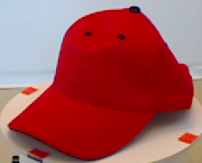
\includegraphics[width=\textwidth]{img/templates/0_crop.png}
		\caption{Rotación $0^{\circ}$}
	\end{subfigure}
	\quad
	\begin{subfigure}[b]{0.25\textwidth}
		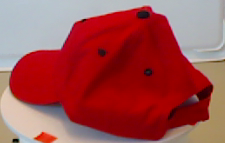
\includegraphics[width=\textwidth]{img/templates/90_crop.png}
		\caption{Rotación $90^{\circ}$}
	\end{subfigure}

	\begin{subfigure}[b]{0.25\textwidth}
		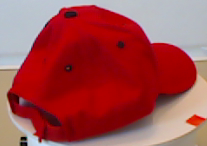
\includegraphics[width=\textwidth]{img/templates/180_crop.png}
		\caption{Rotación $180^{\circ}$}
	\end{subfigure}
	\quad
	\begin{subfigure}[b]{0.25\textwidth}
		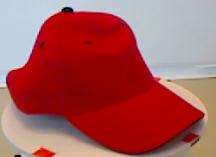
\includegraphics[width=\textwidth]{img/templates/270_crop.png}
		\caption{Rotación $270^{\circ}$}
	\end{subfigure}
	\caption{Templates de una gorra}
	\label{templates_objeto}
\end{figure}

\subsection{Detección}\label{deteccion_rgb}
En esta sección explicaremos el método utilizado para la detección en RGB y la manera de utilizarlo en el esquema de seguimiento propuesto.

\customsubsubsection{Template Matching}
\textit{Template matching} es una técnica del área de procesamiento de imágenes utilizada para encontrar pequeñas partes de una imagen que sean similares a una imagen de referencia (o template). Esta técnica tiene varias aplicaciones que van desde la robótica hasta el control de calidad de piezas manufacturadas.

Para aplicar esta técnica se necesitan tres cosas:
\begin{itemize}
	\item Una imagen de búsqueda: la imagen donde intentaremos encontrar la aparición del template
	\item Una imagen como template: porción de imagen buscada
	\item Método de comparación de imágenes
\end{itemize}

La técnica consiste en ir moviendo el template sobre la imagen de búsqueda píxel por píxel, de izquierda a derecha y de arriba hacia abajo. En cada píxel, se va comparando el template con el área de la imagen de búsqueda que comienza en el píxel explorado y cuyo tamaño es igual al del template. Esta comparación nos indica la similitud que hay entre el área de la imagen de búsqueda y el template. A medida que se recorre la imagen se va acumulando este valor de comparación junto con la posición del píxel en la imagen, hasta haber recorrido toda la imagen.

Una vez recorrida la imagen se busca cual de todas las comparaciones es mejor y se obtiene el píxel donde comienza la región, que junto con el tamaño del template permiten obtener el recuadro de la imagen de búsqueda que más se parece al template.

Existen distintos métodos de comparación de imágenes, cada uno con sus ventajas y desventajas, aunque todos utilizan la comparación píxel por píxel. Uno de los métodos más conocidos es la diferencia cuadrática, que tiene la siguiente fórmula: Sea I la imagen de búsqueda y T el template, la diferencia cuadrática se calcula así:
\begin{equation}\label{eq:diferencia_cuadratica}
R(x, y) = \displaystyle\sum\limits_{x', y'} (T(x', y') - I(x + x', y + y'))^2
\end{equation}

Teniendo en cuenta el método de comparación elegido, una manera de utilizar esta técnica para la detección es definir un umbral para la comparación y aplicar \textit{template matching} entre una imagen y un template. Si el mejor valor de comparación obtenido está por debajo del umbral elegido, se sabe con cierta probabilidad que la detección fue exitosa. Por el contrario, si la comparación está por debajo de ese umbral se asume que se está frente a una detección fallida y se reporta que el template no se encuentra en la imagen.


\customsubsubsection{Esquema de detección}

La información recolectada durante el entrenamiento se toma con la intención de poder aplicar como método de detección al algoritmo de \textit{Template matching}. La implementación utilizada es la que se encuentra presente en la librería \textit{OpenCV} para C++. Esta implementación recibe varios parámetros. El primero es el frame de la escena a donde se desea detectar el objeto. El segundo es el template con el que se va a buscar el objeto. El tercero es opcional y es una máscara para el template del objeto. El último parámetro le indica al algoritmo de template matching que comparación usar para emparejar el template a la imagen. En este trabajo se decide utilizar diferencia cuadrática píxel por píxel normalizada, presente en la fórmula \ref{eq:diferencia_cuadratica}

Pero aplicar este método de manera directa no es suficiente. El problema principal es que la escena de donde se obtienen los templates del objeto a buscar puede no ser la misma escena en la que se realiza el seguimiento. Esto significa que las poses del objeto tomadas en la etapa de entrenamiento pueden ser completamente distintas a las poses del objeto en la escena. Además, la distancia de la cámara al objeto en la escena de búsqueda puede variar y diferir ampliamente de la distancia entre ambos en la escena en donde se capturan los templates del objeto. Por este motivo también puede diferir la escala del objeto en cada escena.

Teniendo en cuenta estos problemas decidimos realizar varias corridas del algoritmo de \textit{template matching}. En primera medida en cada pasada se va modificando template utilizado como parámetro del mismo aprovechando los datos obtenidos en la etapa de entrenamiento. Con esto se ataca de mejor manera el problema de las distintas poses en las que puede estar el objeto en la escena. Además, para que la detección sea más robusta frente a cambios de tamaño del objeto que se desea encontrar se toma a cada uno de los templates y se les aplican varios cambios de escala y se utilizan estas muestras como entrada para el algoritmo de template matching. Una vez corrido el algoritmo para cada template y sus diferentes escalas, se obtiene como resultado final la corrida que tenga menor diferencia cuadrática y que esté por debajo de un umbral predefinido. La información que se almacena como resultado son las coordenadas del cuadrante que contiene al objeto encontrado. Una vez almacenada esta información, el sistema pasa a la etapa de seguimiento.

\subsection{Seguimiento}\label{tracking_rgb}
Como se explicó al comienzo del capítulo, esta etapa consta de seguir al objeto detectado en la etapa anterior frame a frame. Para concretar este objetivo se necesita encontrar una manera de combinar la información obtenida durante las dos etapas anteriores. Existen muchas maneras de llevar a cabo esta tarea. La forma que elegimos para este trabajo fue utilizar un método de comparación por histogramas.

Cada imagen RGB consta de tres imágenes, una por cada canal. Para calcular el histograma de una imagen se toman los distintos valores (intensidad) de cada píxel y se cuenta la cantidad de veces que se repite cada uno de esos valores en la imagen. Las imágenes que utilizamos durante el transcurso de este trabajo son de 8 bits por píxel, por lo que cada píxel puede tomar un valor entre 0 y 255. Para que las comparaciones entre histogramas sean más robustas lo que se decidió fue trabajar con histogramas normalizados.


\begin{figure}
	\centering
	\begin{subfigure}[b]{0.25\textwidth}
		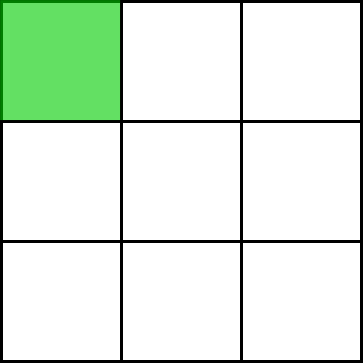
\includegraphics[width=\textwidth]{img/grilla/primercuadrante.png}
		\caption{Primer frame de búsqueda}
		\label{frames_solapados_1}
	\end{subfigure}
	\quad
	\begin{subfigure}[b]{0.25\textwidth}
		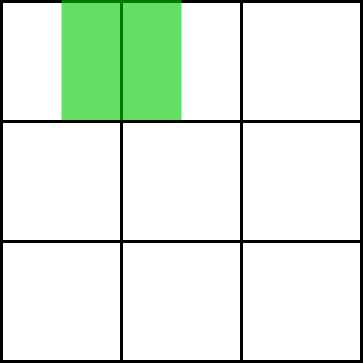
\includegraphics[width=\textwidth]{img/grilla/segundocuadrante.png}
		\caption{Segundo frame de búsqueda}
		\label{frames_solapados_2}
	\end{subfigure}
	\quad
	\begin{subfigure}[b]{0.25\textwidth}
		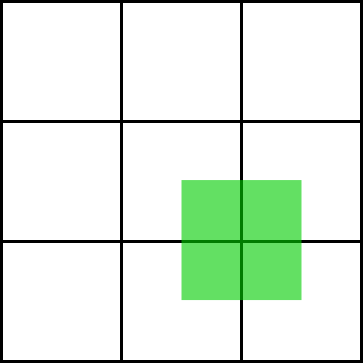
\includegraphics[width=\textwidth]{img/grilla/decimonovenocuadrante.png}
		\caption{$19^{\circ}$ frame de búsqueda}
		\label{frames_solapados_3}
	\end{subfigure}
	\caption{Se busca en cada cuadrante de la grilla y en los recuadros del mismo tamaño que cubren los bordes de la grilla principal}
	\label{frames_solapados}
\end{figure}

El algoritmo de tracking implementado se puede separar en dos partes. Por un lado tenemos el método de búsqueda y por el otro el algoritmo de comparación por histogramas. El método de búsqueda se utiliza para explorar un espacio predefinido en donde se asume estará el objeto en el siguiente frame. Este algoritmo toma un área de tamaño 9 veces mayor a la del cuadrante reportado por el algoritmo de detección respetando el centro del mismo. Luego divide esta área en cuadrantes los que serán utilizados por el algoritmo de comparación para definir si el objeto está o no allí. En la figura \ref{frames_solapados} se muestra una secuencia de búsqueda por cuadrantes. Para hacer más robusta la búsqueda frente a cambios de tamaño del objeto este mismo método de búsqueda por cuadrantes se realiza varias veces cambiando el tamaño del cuadrante.

La segunda parte del algoritmo de tracking consta en definir cuál de todos los cuadrantes explorados en la etapa de búsqueda es el que contiene el objeto que se está buscando o, en caso de fallar en la búsqueda, indicar que el objeto no se encontró en el frame. Con este objetivo, se compara el histograma de cada uno de los cuadrantes explorados con el cuadrante del frame anterior en donde se reportó haber encontrado el objeto. Para ello se toma de cada recuadro el histograma de los canales S y V del esquema de colores HSV y se los compara utilizando la distancia de \textit{Bhattachayyra}, cuya definición es: Sean $H_1$ y $H_2$ los dos histogramas a comparar, la distancia de Bhattachayyra $d(H_1, H_2)$ se calcula a través de la siguiente fórmula:

\begin{equation}
	d(H_1, H_2) = \sqrt{1 - \frac{1}{\sqrt{\bar{H_1} \bar{H_1} N^2}} \sum_I \sqrt{H_1(I) \cdot H_2(I)}}
\end{equation}

donde

$$
	\bar{H_k} = \frac{1}{N} \sum_J H_k(J)
$$

y $N$ es la cantidad de bines del histograma.

Como resultado de estas comparaciones se obtiene un cuadrante cuyo valor de comparación con el del frame anterior es inferior a cierto umbral dado. Si ninguno de los cuadrantes tiene un valor comparativo menor al umbral el algoritmo indica que el objeto no fue encontrado, motivo por el cual se debe volver a la etapa de detección.

El problema con esta aproximación es que al estar basada únicamente en el recuadro encontrado en el frame anterior el objeto puede ir quedando de a poco fuera del recuadro resultante hasta quedar completamente fuera del mismo. Esto puede suceder ya que la diferencia entre dos cuadrantes resultantes sucesivos es relativamente baja. Cuando esto sucede el algoritmo va a seguir reportando al objeto como encontrado aunque el área reportada no incluya ninguna parte del mismo.

Para evitar este inconveniente se realiza una doble comparación de histogramas. Además de la comparación antes mencionada, se compara el histograma de cada cuadrante de búsqueda con el histograma de uno de los templates del objeto obtenido en la etapa de entrenamiento. En este caso la comparación se realiza utilizando el esquema RGB, calculando el histograma para los tres canales.

\begin{figure}
	\centering
	\begin{subfigure}[b]{0.3\textwidth}
		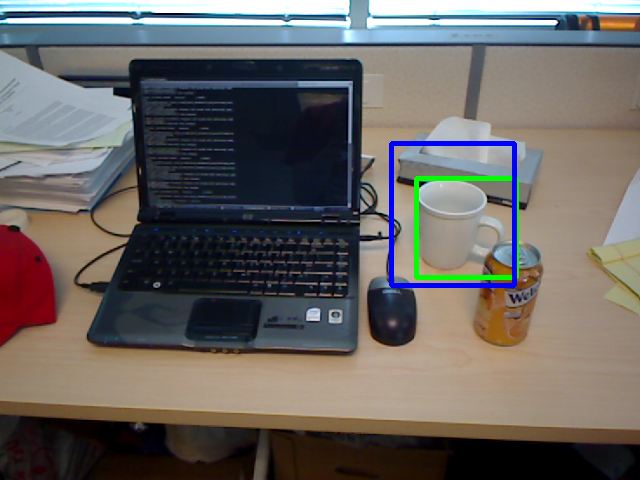
\includegraphics[width=\textwidth]{img/seguimiento_solo_frame/solo_frame-desk_1-coffee_mug_5-frame_26.png}
	\end{subfigure}
	\begin{subfigure}[b]{0.3\textwidth}
		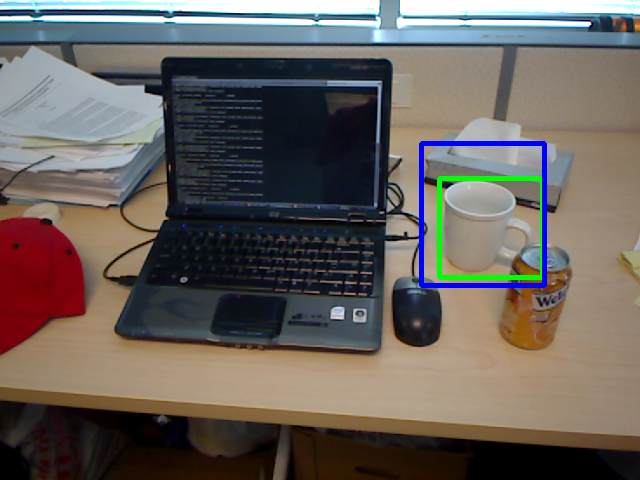
\includegraphics[width=\textwidth]{img/seguimiento_solo_frame/solo_frame-desk_1-coffee_mug_5-frame_27.png}
	\end{subfigure}
	\begin{subfigure}[b]{0.3\textwidth}
		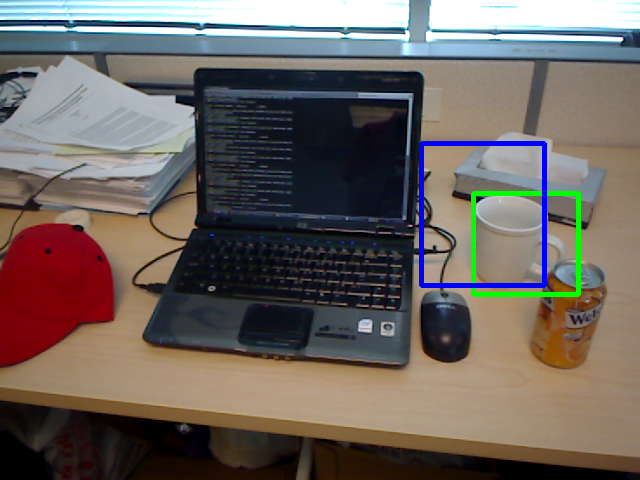
\includegraphics[width=\textwidth]{img/seguimiento_solo_frame/solo_frame-desk_1-coffee_mug_5-frame_28.png}
	\end{subfigure}


	\begin{subfigure}[b]{0.3\textwidth}
		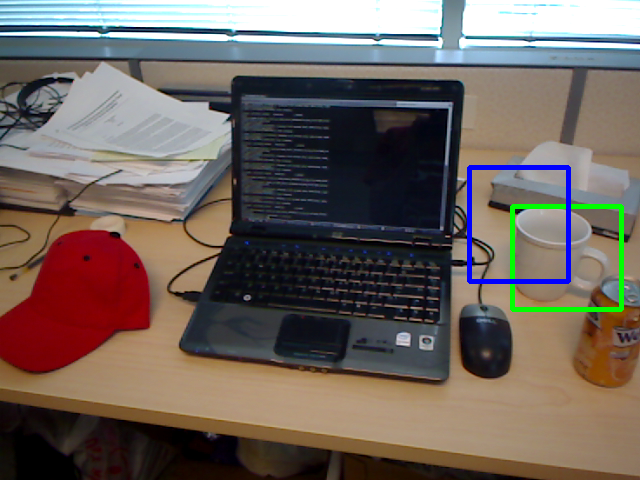
\includegraphics[width=\textwidth]{img/seguimiento_solo_frame/solo_frame-desk_1-coffee_mug_5-frame_29.png}
	\end{subfigure}
	\begin{subfigure}[b]{0.3\textwidth}
		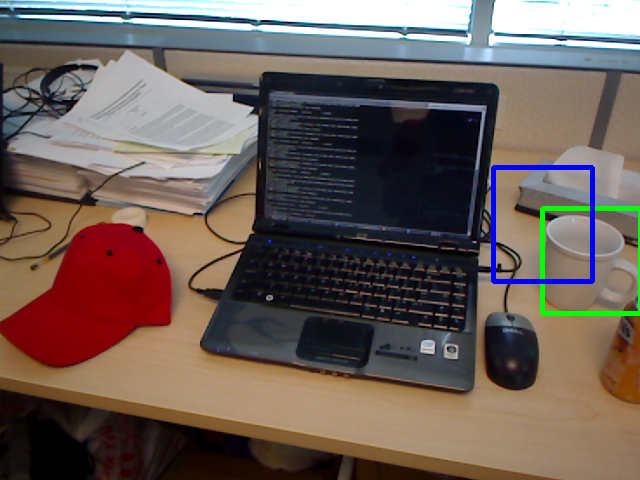
\includegraphics[width=\textwidth]{img/seguimiento_solo_frame/solo_frame-desk_1-coffee_mug_5-frame_30.png}
	\end{subfigure}
	\begin{subfigure}[b]{0.3\textwidth}
		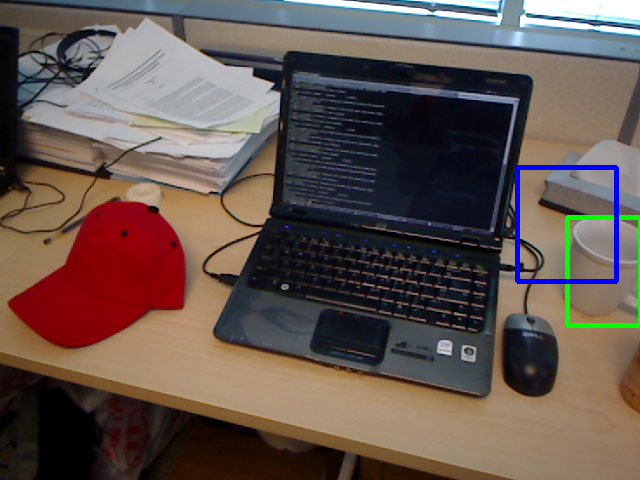
\includegraphics[width=\textwidth]{img/seguimiento_solo_frame/solo_frame-desk_1-coffee_mug_5-frame_31.png}
	\end{subfigure}

	\begin{subfigure}[b]{0.3\textwidth}
		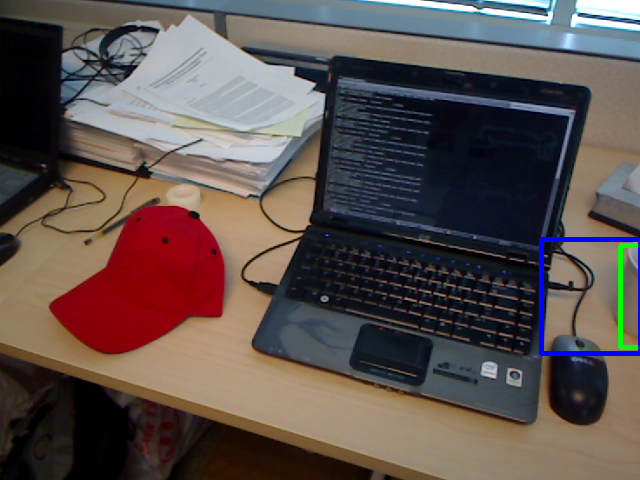
\includegraphics[width=\textwidth]{img/seguimiento_solo_frame/solo_frame-desk_1-coffee_mug_5-frame_32.png}
	\end{subfigure}
	\begin{subfigure}[b]{0.3\textwidth}
		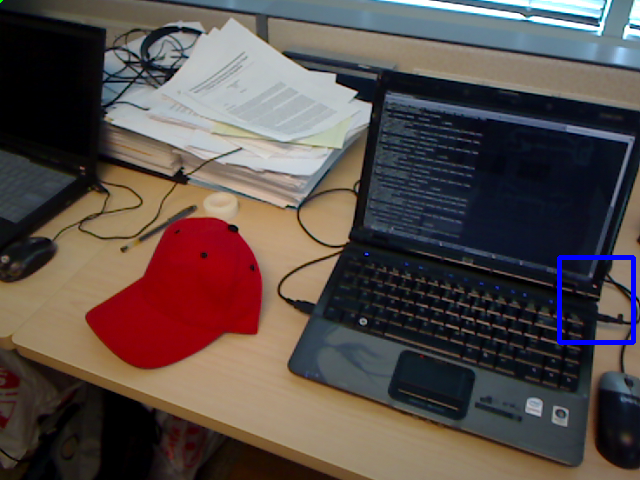
\includegraphics[width=\textwidth]{img/seguimiento_solo_frame/solo_frame-desk_1-coffee_mug_5-frame_33.png}
	\end{subfigure}
	\begin{subfigure}[b]{0.3\textwidth}
		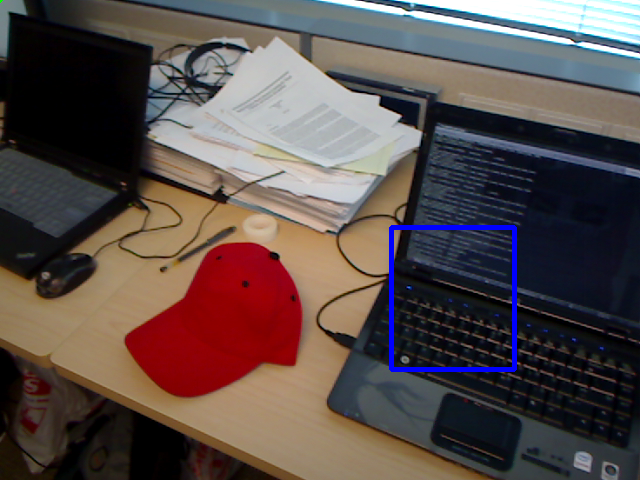
\includegraphics[width=\textwidth]{img/seguimiento_solo_frame/solo_frame-desk_1-coffee_mug_5-frame_34.png}
	\end{subfigure}

	\caption{Seguimiento frame a frame divergiendo. Aquí se estaba usando solo comparación de histogramas entre el frame anterior y el actual}
	\label{frame_only_tracking}
\end{figure}


\begin{figure}
	\centering
	\begin{subfigure}[b]{0.3\textwidth}
		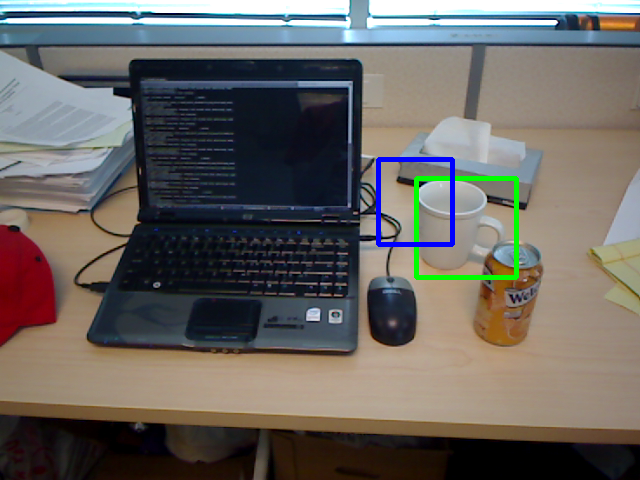
\includegraphics[width=\textwidth]{img/seguimiento_frame_template/frame_template-desk_1-coffee_mug_5-frame_26.png}
	\end{subfigure}
	\begin{subfigure}[b]{0.3\textwidth}
		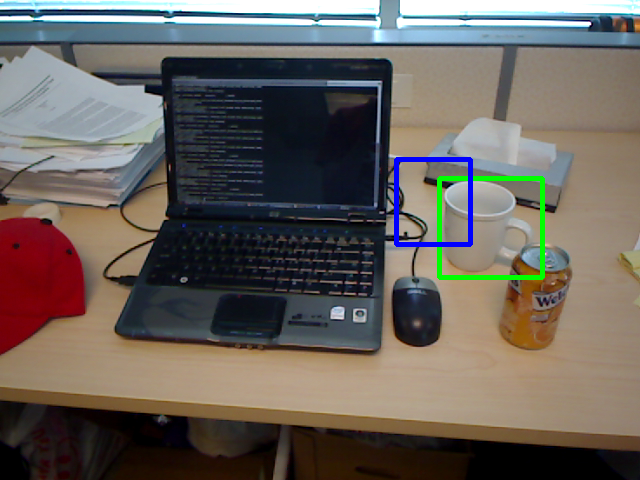
\includegraphics[width=\textwidth]{img/seguimiento_frame_template/frame_template-desk_1-coffee_mug_5-frame_27.png}
	\end{subfigure}
	\begin{subfigure}[b]{0.3\textwidth}
		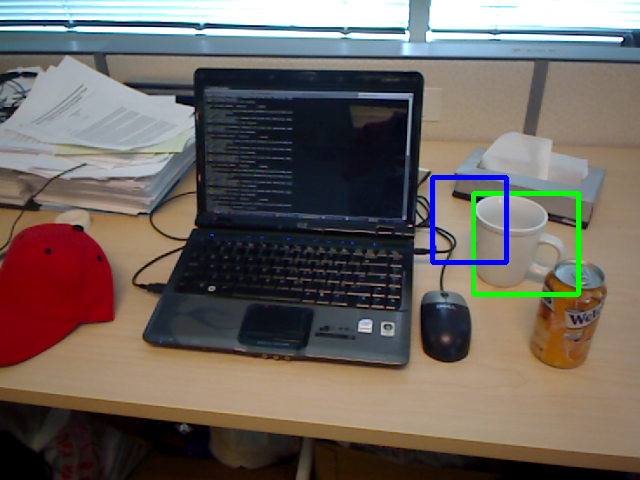
\includegraphics[width=\textwidth]{img/seguimiento_frame_template/frame_template-desk_1-coffee_mug_5-frame_28.png}
	\end{subfigure}


	\begin{subfigure}[b]{0.3\textwidth}
		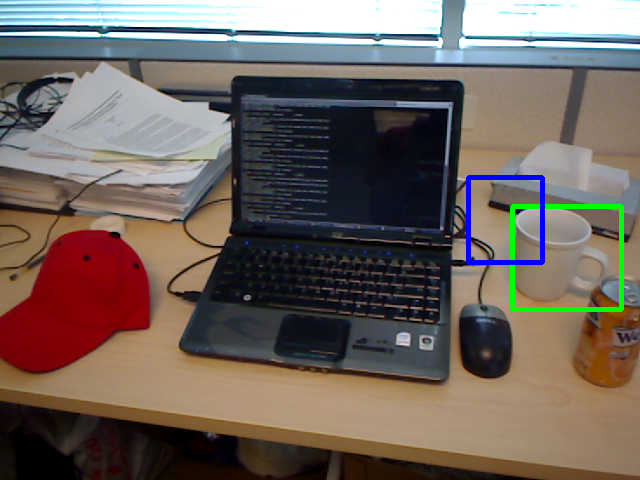
\includegraphics[width=\textwidth]{img/seguimiento_frame_template/frame_template-desk_1-coffee_mug_5-frame_29.png}
	\end{subfigure}
	\begin{subfigure}[b]{0.3\textwidth}
		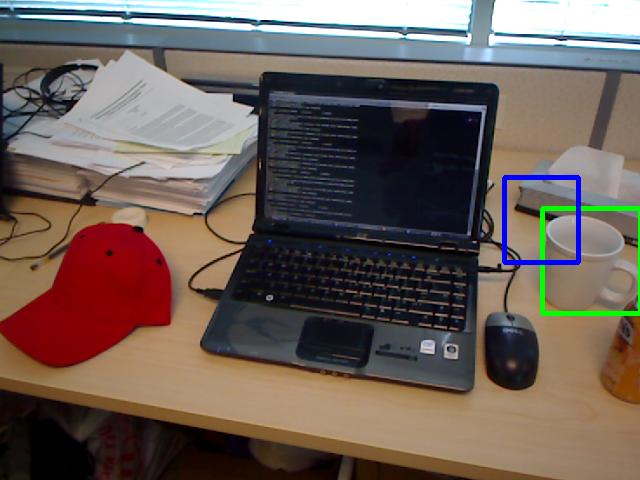
\includegraphics[width=\textwidth]{img/seguimiento_frame_template/frame_template-desk_1-coffee_mug_5-frame_30.png}
	\end{subfigure}
	\begin{subfigure}[b]{0.3\textwidth}
		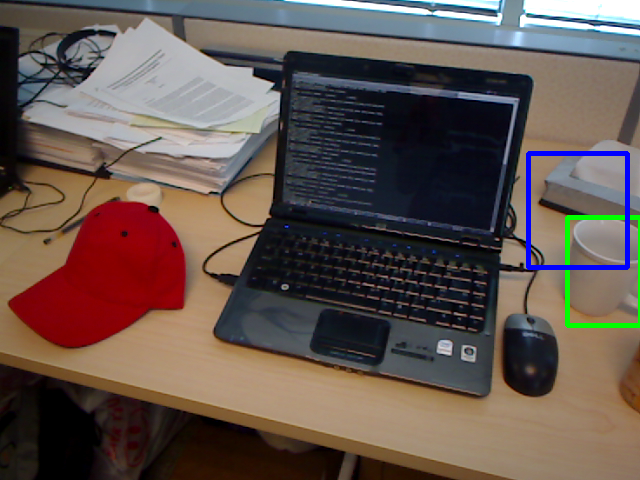
\includegraphics[width=\textwidth]{img/seguimiento_frame_template/frame_template-desk_1-coffee_mug_5-frame_31.png}
	\end{subfigure}

	\begin{subfigure}[b]{0.3\textwidth}
		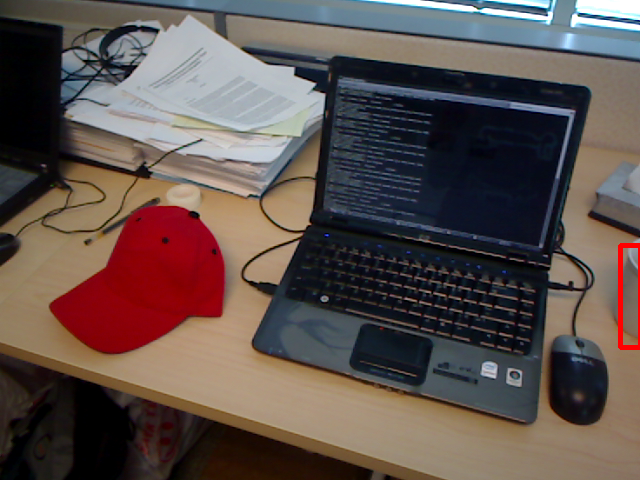
\includegraphics[width=\textwidth]{img/seguimiento_frame_template/frame_template-desk_1-coffee_mug_5-frame_32.png}
	\end{subfigure}
	\begin{subfigure}[b]{0.3\textwidth}
		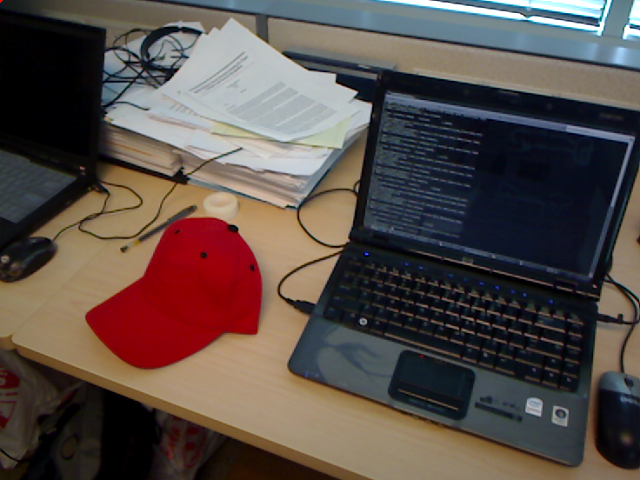
\includegraphics[width=\textwidth]{img/seguimiento_frame_template/frame_template-desk_1-coffee_mug_5-frame_33.png}
	\end{subfigure}
	\begin{subfigure}[b]{0.3\textwidth}
		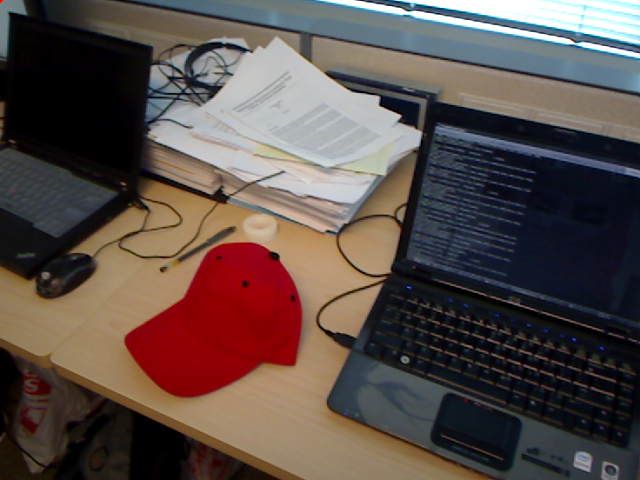
\includegraphics[width=\textwidth]{img/seguimiento_frame_template/frame_template-desk_1-coffee_mug_5-frame_34.png}
	\end{subfigure}

	\caption{Seguimiento frame a frame sin falsos positivos. Aquí se estaba usando las comparaciones de histogramas entre el frame anterior, el actual y el template del objeto}
	\label{frame_template_tracking}
\end{figure}


En las figuras \ref{frame_only_tracking} y \ref{frame_template_tracking} se pueden ver dos secuencias del algoritmo de seguimiento, una con comparación de histogramas únicamente entre frame y frame y otra que agrega además la comparación con el template del objeto respectivamente. El cuadrante de color verde indica la ubicación del objeto en la escena según el ground truth, en este caso, una taza. El cuadrante de color azul es el reportado por nuestro algoritmo. En la Figura \ref{frame_only_tracking} podemos ver como frame a frame el cuadrante azul se aleja de la taza frame a frame hasta que en el frame 8 de este extracto de la escena el algoritmo indica que encontró a la taza en una zona que en realidad es parte de la notebook. En la Figura \ref{frame_template_tracking} podemos ver en cambio que el área reportada por el algoritmo se mantiene más estable. En el frame 7 aparece un recuadro rojo. Eso significa que el algoritmo de seguimiento perdió el rastro del objeto y en ese frame hizo falta correr el algoritmo de detección. Luego, en los frames 8 y 9 el algoritmo no reporta haber seguido al objeto. Por este motivo es que se utiliza la doble comparación de histogramas, tanto con el frame anterior como con el template del objeto.

Una vez corridas estas dos sub-etapas dentro de la etapa de seguimiento, pueden ocurrir dos cosas: si el algoritmo reporta al objeto como encontrado, se almacenan los datos necesarios y se continúa con el algoritmo de seguimiento en el frame siguiente. En cambio, si el algoritmo indica que el objeto no se encuentra en el frame se vuelve a la etapa de detección explicada previamente.






\section{Método propuesto para profundidad}\label{metodo_d}
En esta sección explicaremos los métodos utilizados durante las distintas etapas del esquema propuesto para el seguimiento en profundidad, entre los que se encuentra un método de estimación de pose proveniente del trabajo \cite{6630856}, el cual fue utilizado en gran parte de esta tesis, así como también un método de alineación de formas 3D, llamado \textit{Iterative Closest Point} (ICP). Además, al igual que se hizo en la Sección \ref{metodo_rgb} se detalla para cada etapa del algoritmo como se utiliza cada método y de que manera se los une para formar el sistema de seguimiento.


\subsection{Iterative Closest Point (ICP)}\label{ICP}
En esta sección explicaremos el método de alineación de formas 3D, llamado \textit{Iterative Closest Point} (ICP) surgido en el trabajo \cite{besl1992method}. En este trabajo se intenta encontrar respuesta a uno de los principales problemas en visión en computación: dada cierta información 3D en un sistema de coordenadas de un sensor, que describe una forma que puede corresponder a un modelo y dado un modelo en una representación geométrica distinta, lograr estimar la rotación y traslación óptimas que permitan alinear las dos formas minimizando la distancia entre ambas, permitiendo así determinar la equivalencia de las mismas usando \textit{mean-square} como métrica de distancia.

El algoritmo presentado puede ser utilizado en múltiples tipos de representaciones de datos geométricos como conjunto de puntos, conjuntos de segmentos de líneas, curvas paramétricas, superficies paramétricas, etc. Además se puede utilizar cualquier otra representación siempre que se acompañe a la misma de un método para calcular el punto más cercano de esa forma a un punto dado. Además de necesitar una manera de calcular el punto más cercano, también es necesario un método para obtener la rotación y traslación de mínimos cuadrados.

A continuación presentamos el pseudocódigo para el algoritmo ICP:

%\newpage
% \footnotesize
% \lstinputlisting[language=Python, frame=single, float]{icp_pseudocode.py}
% \normalsize

\begin{algorithm}
\caption{Pseudocódigo ICP}
\label{lst:icp}
\begin{algorithmic}
\Function{icp}{$obj\_points$, $scene\_points$}
	\State $t \gets TRANSFORMACION\_IDENTIDAD$
	\State $t\_obj \gets obj\_points$
	\State $sq\_error \gets MAX\_INT$
	\While{$no\ se\ cumplen\ condiciones\ de\ corte$}
		\State $closest\_points \gets get\_closest\_points$($t\_obj$, $scene\_points$)
		\State $new\_t \gets get\_transformation$($closest\_points$) \Comment{i.e: SVD}
		\State $t\_obj$ = transformar($t\_obj$, $new\_t$)
		\State $sq\_dist \gets mean\_sq\_dist$($t\_obj$, $scene$)
		\If{$abs(sq\_error,\ sq\_dist) < umbral\_de\_error$}
			\State break \Comment{Salir del while}
		\EndIf
		\State $sq\_error \gets sq\_dist$
	\EndWhile

    \State \Return $t\_obj$, $sq\_error$
\EndFunction
\end{algorithmic}
\end{algorithm}

Entre las condiciones de corte para este algoritmo hay un límite máximo para la cantidad de iteraciones, el que se encuentra en el pseudocódigo que corta en caso de que dos transformaciones sucesivas difieran en el error cuadrático en menos de un umbral dado y por último una condición parecida que verifica que el error cuadrático de una transformación obtenida sea menor a un umbral.


En este mismo trabajo, además de presentar este algoritmo, se demuestra que el mismo converge monótonamente hacia un mínimo local con respecto a la distancia cuadrática media. Sin embargo, nada puede decirse sobre la convergencia hacia el mínimo global deseado.

Notar que el algoritmo no es útil si solo un subconjunto de los puntos se corresponde con el modelo o con un subconjunto del modelo. Lamentablemente esto sucede con la mayoría de los algoritmos de ``pareo'' de formas en 3D. Pero sigue resultando útil si todo el conjunto de puntos se corresponde con parte del modelo.

Entre las ventajas más importantes de este método está el hecho de que maneje los seis grados de libertad y que sea independiente de la forma de representación. Además, no requiere de extracción de descriptores y puede ser fácilmente utilizado en conjunto con otros algoritmos. Por otro lado, una desventaja importante es que es susceptible a outliers. Esto tiene como extensión que el algoritmo no sirve para resolver el problema de segmentar objetos en una escena.


\subsection{Alineación de objetos rígidos en una escena}\label{alignment_prerejective}
El problema de determinar una transformación que permita alinear dos superficies ha generado muchas investigaciones en el campo de la visión en computación. Desde la manipulación de objetos en robótica hasta la reconstrucción de un modelo de un objeto o escena a partir de varias imágenes tomadas de distintos ángulos. En general estos métodos requieren una solución precisa para luego poder utilizar el resultado con otros problemas de procesamiento.

Hay muchos métodos conocidos para resolver este problema tanto en el dominio 2D como en el 3D y en general están basados en extracción de descriptores para eliminar falsas correspondencias entre las dos superficies o modelos. Es ampliamente conocido el hecho que los descriptores locales proveen una alta estabilidad dada su tolerancia al ruido y oclusiones. El objetivo del trabajo \cite{6630856} es combinar entradas del dominio RGB o 2D y de profundidad o 3D de manera eficiente para resolver el problema de la estimación de pose.

En este trabajo se realizan una serie de pasos bien definidos hasta obtener una transformación como resultado final que indique la pose del objeto en la escena. En primera instancia, se obtiene un conjunto de puntos de interés utilizando un sistema de \textit{Early Cognitive Vision} (ECV). Los descriptores provenientes de este sistema ECV son considerados atómicos y se los llama \textit{primitivos}. La densidad de estos descriptores está en un punto intermedio entre una imagen con puntos de interés escasos y descriptores de formas en 3D muy densos. Cada una de estas primitivas tiene información geométrica y de texturas de manera que sirve como descriptor para imágenes RGB, para nubes de puntos o para una combinación de ambas. Este sistema permite clasificar regiones de una imagen en tres categorías: región homogénea, región de borde y región con textura. En este trabajo se usan solo las últimas dos categorías ya que los píxeles en las regiones homogéneas resultan ser ambiguos para buscar correspondencias.
A cada punto de interés se le agrega un descriptor que contempla información de textura y geometría del objeto en una vecindad de puntos predefinida para aumentar la habilidad del método para distinguir falsas correspondencias. A esto se lo llama \textit{ECV context descriptors}.

Una vez obtenidos los puntos de interés y sus descriptores tanto en el objeto como en la escena se utiliza \textit{RANSAC} \cite{ransac} para estimar una transformación que alinee el objeto con la escena. Formalmente lo que se busca es una transformación $\hat{T}$ que minimice la suma de la diferencia de cuadrados entre los puntos p del modelo del objeto P y sus correspondencias con los puntos q en la escena Q:

\begin{equation}\label{eq:mindif}
\hat{T} = \argmin_T \varepsilon(T) = \argmin_T \sum_{p \in P}(Tp - q)^2
\end{equation}

A continuación presentamos el pseudocódigo de la heurística RANSAC de este trabajo:
%\newpage
% \footnotesize
% \lstinputlisting[language=Python, frame=single, float]{alignment_prerejective_pseudocode.py}
% \normalsize
\begin{algorithm}
\caption{Pseudocódigo de la heurística de alineación de objetos rígidos}
\label{lst:icp}
\begin{algorithmic}
\Function{$alignment\_prerejective$}{$obj\_data$, $scene\_data$}
	\State $best\_value \gets MAX\_INT$
	\State $best\_t \gets TRANSFORMACION\_IDENTIDAD$
	\State $obj\_desc \gets ecv\_context\_descriptors(obj\_data)$
    \State $scene\_desc \gets  ecv\_context\_descriptors(scene\_data)$
	\While{$queden\ iteraciones$} \Comment{RANSAC}
		\State // Paso 1
        \State $rand\_desc \gets tomar\_n\_random(obj\_desc)$
        \State $corresp \gets find\_correspondences(scene\_desc, rand\_desc)$
        \State // Paso 2: Descarte rapido si no son isometricos
        \If{\textbf{not} $poligonos\_son\_isometricos(rand\_desc, corresp)$ }
			\State continue \Comment{Ir a siguiente iteracion}
		\EndIf

        \State // Paso 3
		\State $t \gets estimar\_transformacion(rand\_desc, corresp)$
        \State // Paso 4
        \State $t\_obj \gets transformar(obj\_data, t)$
        \State // Paso 5
        \State $pares\_de\_inliers \gets get\_closest\_points(t\_obj, scene\_data)$
        \If {$len(pares\_de\_inliers) < umbral\_inliers$}
			\State continue \Comment{Ir a siguiente iteracion}
		\EndIf
        \State // Paso 6
        \State $sq\_dist \gets mean\_sq\_dist(pares\_de\_inliers)$
        \If {$sq\_dist < best\_value$}
            \State $best\_value \gets sq\_dist$
			\State $best\_t = t$
		\EndIf
	\EndWhile

    \State \Return $best\_t, best\_value$
\EndFunction
\end{algorithmic}
\end{algorithm}


El parámetro de corte aquí presentado es la cantidad de iteraciones, pero también se puede tomar como corte si la diferencia de cuadrados es menor que un umbral dado. La utilización del esquema RANSAC garantiza que el método sea robusto frente a outliers.

En este trabajo se agrega un paso novedoso a este esquema RANSAC, que es el paso 2 marcado en el pseudocódigo. Este paso asume una propiedad geométrica de objetos rígidos para descartar rápidamente malas correspondencias. En particular utilizan el hecho que las distancias entre objetos isométricos en un espacio 3D se mantienen al aplicar transformaciones a esos objetos y hacen un chequeo de las diferencias entre las distancias de los bordes del polígono virtual formado por los puntos random tomados en el paso 1 tanto para el objeto como para la escena. Utilizando una medida de distancia entre estos valores y un umbral descartan rápidamente malas correspondencias. Si se asume que no se descartan potenciales poses que alinean bien los modelos, se obtiene la misma probabilidad de éxito de manera mucho más rápida. Notar que al tomar puntos de manera random este método es en realidad una heurística. Es esperable entonces que para dos corridas del método con mismos datos de entrada se obtengan dos resultados distintos.

Este método puede ser utilizado como paso previo a ICP o en su reemplazo. Ambos métodos cumplen el mismo objetivo de buscar una transformación que alinee dos nubes de puntos permitiendo estimar la pose de una nube con respecto a la otra. Sin embargo poseen características distintas que los hacen destacarse en distintos contextos o condiciones.

\subsection{Entrenamiento}
Esta primera etapa consiste en obtener un modelo del objeto en forma de nube de puntos que pueda ser utilizado en las siguientes etapas. Hay distintas maneras de obtener este modelo y por lo tanto distintas calidades de modelos a obtener. Cuanto más completo sea el modelo, mayor es el tiempo necesario para obtenerlo.

Llamamos vista del objeto a una nube de puntos del mismo tomada desde algún ángulo cualquiera. Esta nube es incompleta ya que no va a incluir las zonas del objeto que no son capturadas por el sensor RGB-D, por ejemplo, la parte de atrás del objeto. Una vista entonces es el modelo más sencillo que se puede obtener para un objeto.

Para obtener un modelo más completo del objeto hay distintas opciones. Una de ellas es generar un modelo CAD y transformarlo a nube de puntos. Otra opción es tomar muchas vistas distintas del objeto, variando altura desde donde se toma captura al objeto y a la vez rotando alrededor del mismo. Luego, estas vistas pueden alinearse usando métodos como los de las secciones \ref{alignment_prerejective} y \ref{ICP} para generar una única nube de puntos del objeto casi tan completa como la que se puede obtener con un modelo CAD.

En la Figura \ref{fig:nube_completa} se muestra una nube de puntos completa desde cuatro ángulos distintos de un mismo muñeco con forma de chef de porcelana. En la Figura \ref{fig:nube_simple} se muestra desde distintos ángulos una nube de puntos tomada desde una única vista de un objeto, en este caso una taza, a modo de ilustrar como se ve una nube incompleta.

\begin{figure}[t]
	\centering
	\begin{subfigure}[b]{0.4\textwidth}
		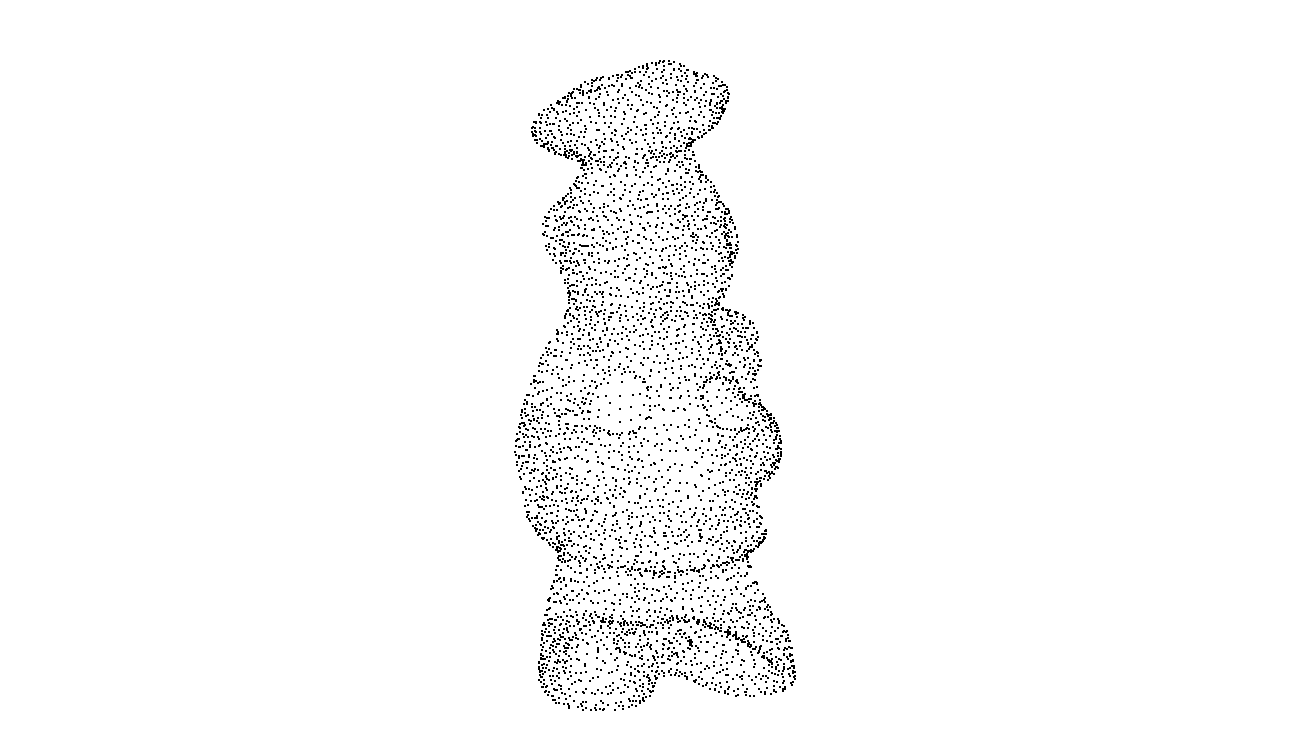
\includegraphics[width=\textwidth]{img/ejemplos_nubes/chef_01.png}
	\end{subfigure}
	\quad
	\begin{subfigure}[b]{0.4\textwidth}
		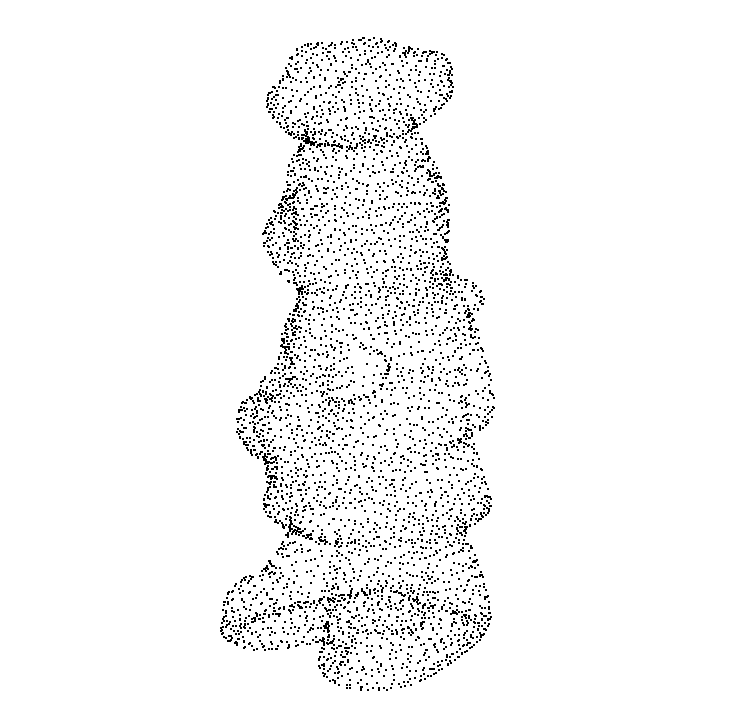
\includegraphics[width=\textwidth]{img/ejemplos_nubes/chef_02.png}
	\end{subfigure}

	\begin{subfigure}[b]{0.4\textwidth}
		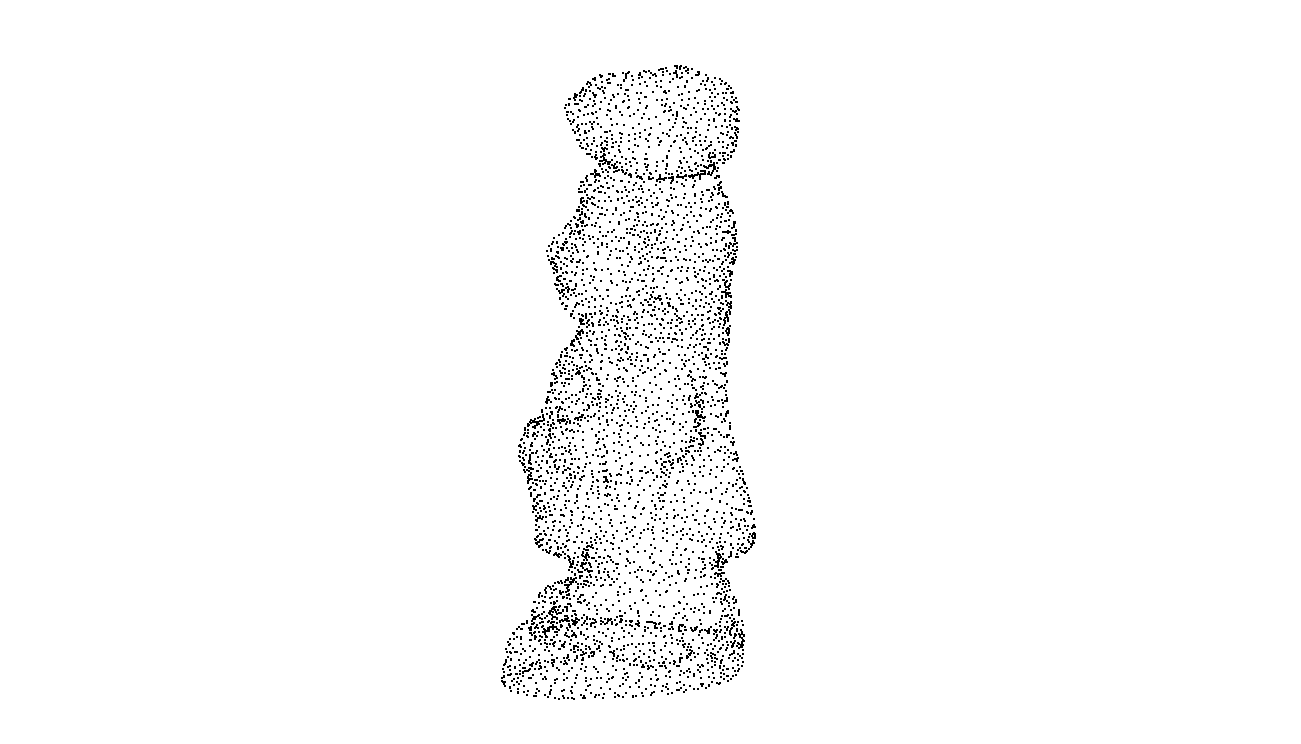
\includegraphics[width=\textwidth]{img/ejemplos_nubes/chef_03.png}
	\end{subfigure}
	\quad
	\begin{subfigure}[b]{0.4\textwidth}
		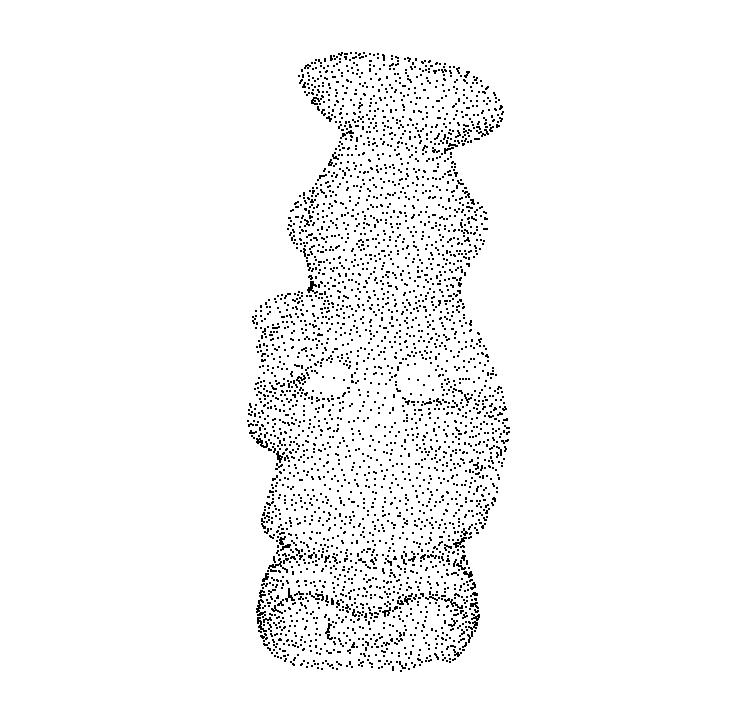
\includegraphics[width=\textwidth]{img/ejemplos_nubes/chef_04.png}
	\end{subfigure}
	\caption{Nube de puntos completa de chef hecho en porcelana.}
	\label{fig:nube_completa}
\end{figure}

\begin{figure}[t]
	\centering
	\begin{subfigure}[b]{0.4\textwidth}
		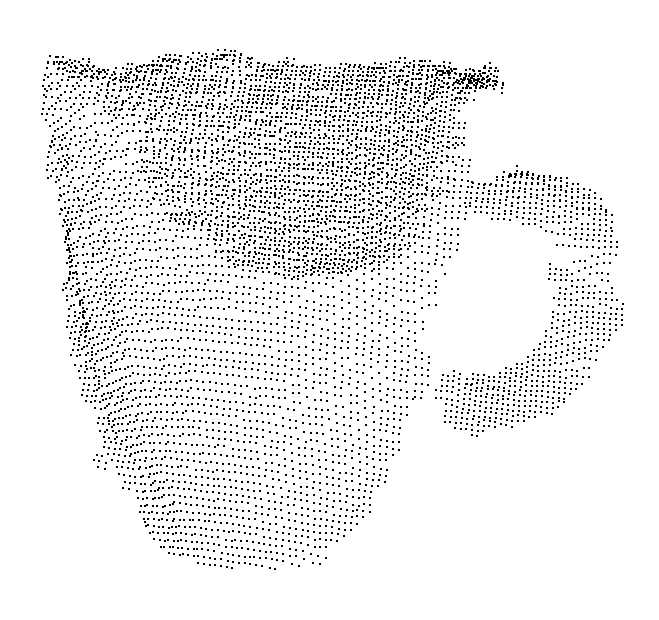
\includegraphics[width=\textwidth]{img/ejemplos_nubes/taza_01.png}
	\end{subfigure}
	\quad
	\begin{subfigure}[b]{0.4\textwidth}
		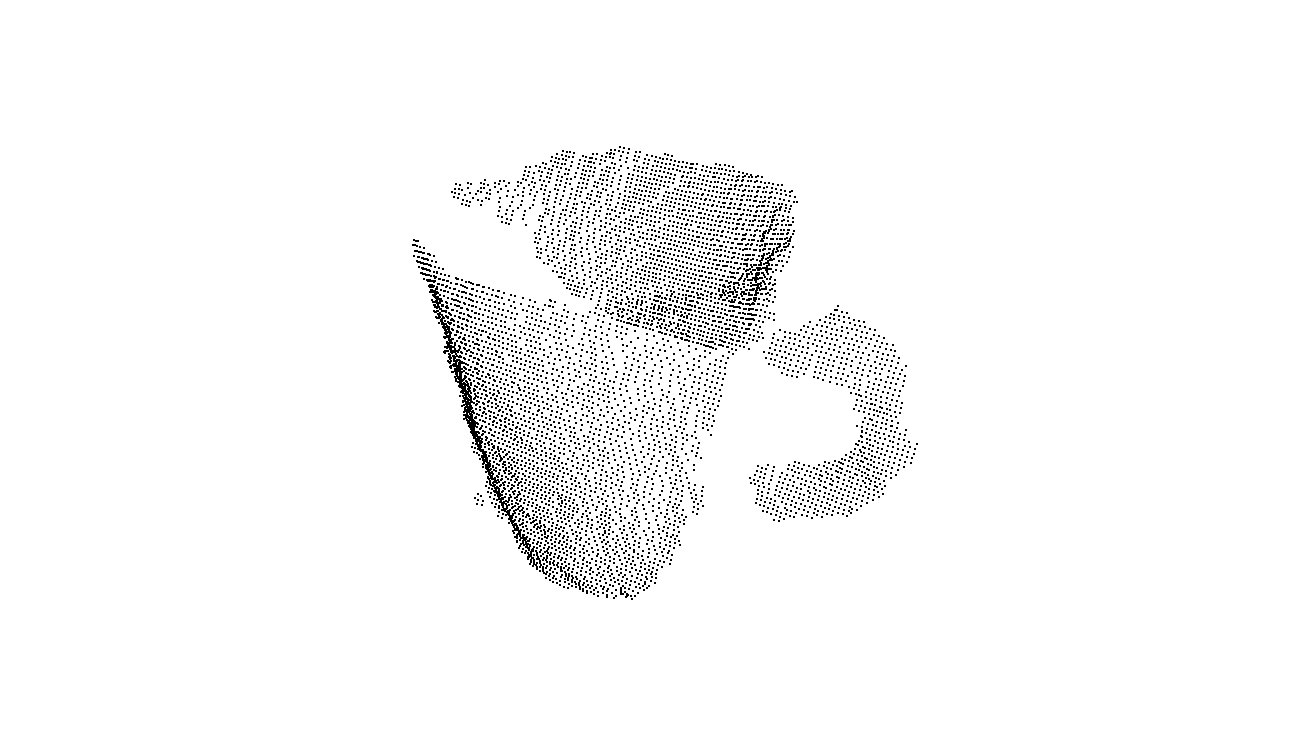
\includegraphics[width=\textwidth]{img/ejemplos_nubes/taza_02.png}
	\end{subfigure}

	\begin{subfigure}[b]{0.4\textwidth}
		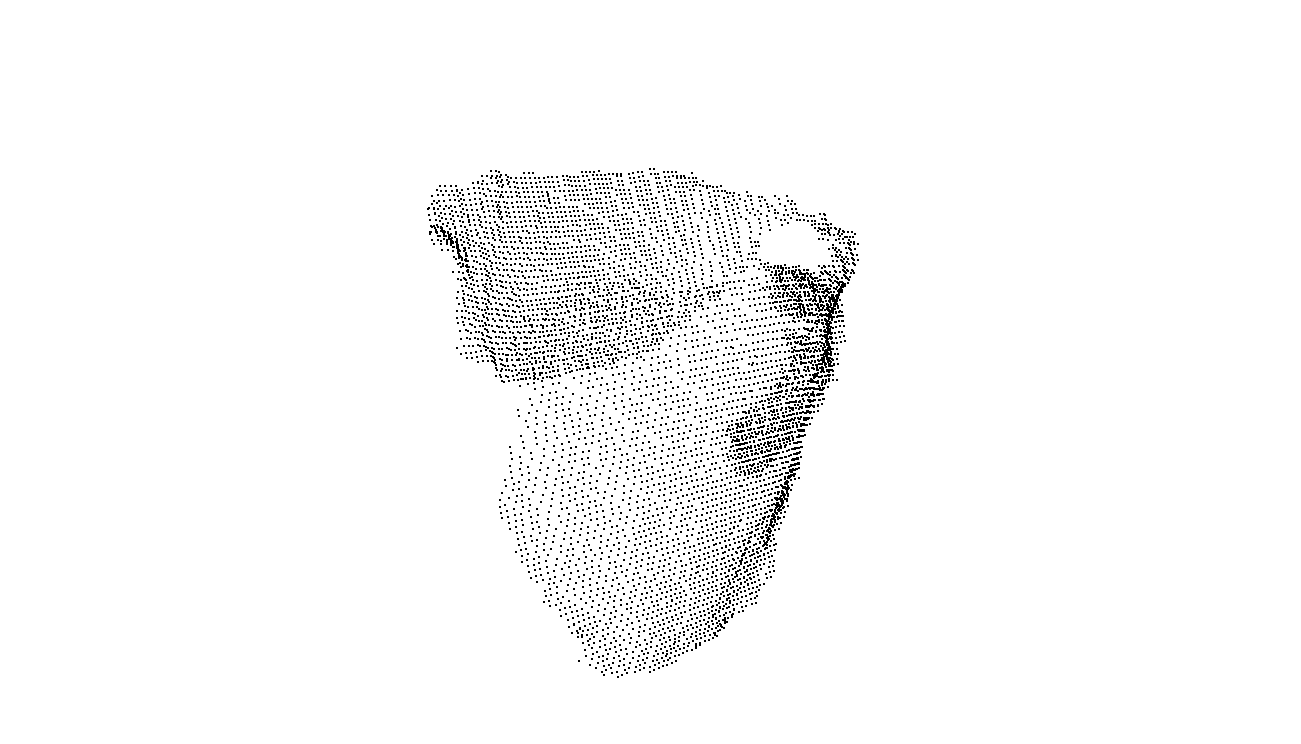
\includegraphics[width=\textwidth]{img/ejemplos_nubes/taza_03.png}
	\end{subfigure}
	\quad
	\begin{subfigure}[b]{0.4\textwidth}
		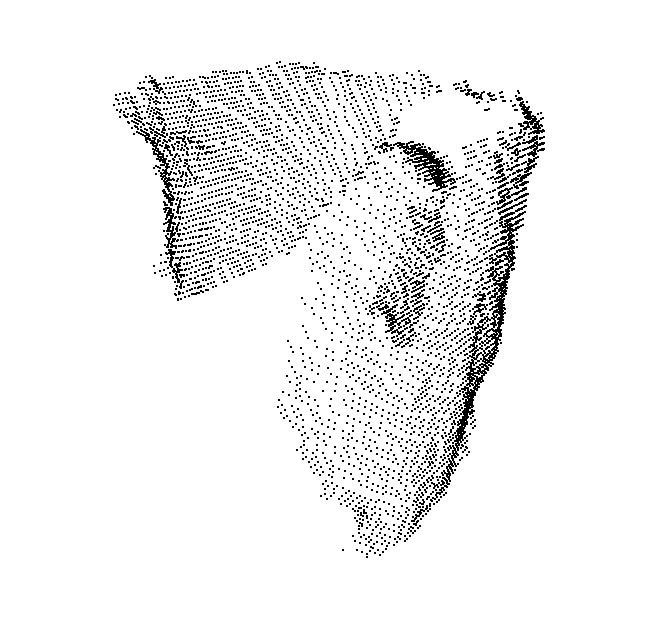
\includegraphics[width=\textwidth]{img/ejemplos_nubes/taza_04.png}
	\end{subfigure}

	\caption{Nube de puntos de una sola vista de una taza.}
	\label{fig:nube_simple}
\end{figure}

Dado que en este trabajo priorizamos la etapa del tracking y que uno de los objetivos es tener un sistema de seguimiento fácilmente adaptable y, en un futuro, lograr un seguimiento en tiempo real, optamos por el método más simple y rápido que es tomar como modelo una nube de puntos de una única vista del objeto. Dependiendo del ángulo y altura desde donde se tome la vista del objeto se puede obtener un modelo más o menos completo. Por ejemplo, en el caso de la taza es conveniente tomar su modelo desde una altura considerable en donde se vea parte del interior de la taza y todo el frente. De esta manera se obtiene mucha información sobre la forma y profundidad de la misma y esto beneficia al funcionamiento de las siguientes etapas.

Este entrenamiento es similar al necesario en RGB para luego poder utilizar template matching en la detección. Utilizar como modelo una vista del objeto a seguir es comparable a obtener un template RGB del objeto. Ambas formas proveen una información parcial sobre el objeto en donde solo se conoce una porción del mismo.

Una vez almacenada esta información se continúa con la siguiente etapa del sistema: la detección.

\subsection{Detección}\label{deteccion_d}
En la segunda etapa se utiliza el método descripto en la Sección \ref{alignment_prerejective} refinando el resultado con ICP (ver Sección \ref{ICP}). La elección del mismo se realizó luego de correr varias pruebas que corroboraran su factibilidad. Durante estas pruebas se obtuvieron malos resultados cuando se corría el algoritmo para un objeto en una nube de puntos de un frame proveniente de una secuencia de video RGB-D. Sin embargo, si se tomaba solo una sección de esa nube de puntos en donde entre otras cosas estaba el objeto buscado la detección funcionaba correctamente y con mucha precisión.

Teniendo en cuenta esto se pensó en una variante para la detección que utilice el método elegido. Esta tiene como primer paso obtener el alto y el ancho de la nube de puntos tomada como modelo del objeto a seguir durante el entrenamiento. Luego se divide la escena en cuadrantes cuyo tamaño es el doble de ancho y alto que el del modelo y se corre el método de detección en cada cuadrante. Con el fin de detectar el objeto cuando el mismo se extiende sobre dos o más regiones, la búsqueda se hizo utilizando un marco que recorre todos los cuadrantes y sus uniones, como puede observarse en la figura \ref{frames_solapados}. Notar que la división por cuadrantes solo se realizó en los ejes ``x'' e ``y'' y no en el eje ``z''. La detección se corre en cada uno de estos cuadrantes y puede suceder que:
\begin{itemize}
	\item No se encontró el objeto en ningún cuadrante: en este caso el algoritmo indica que el objeto no se encuentra en el frame
	\item Se encontró el objeto en un cuadrante
	\item Se encontró el objeto en varios cuadrantes: el algoritmo devuelve la mejor posición encontrada según un puntaje de buena alineación devuelto por el algoritmo de la Sección \ref{alignment_prerejective}.
\end{itemize}

Si la detección es positiva, se refina la alineación corriendo ICP entre el modelo del objeto transformado por el primer método y el cuadrante de la escena donde fue encontrado. Con el objetivo de comenzar el seguimiento en las mejores condiciones posibles, se intentan tomar los puntos del objeto buscado pertenecientes a la escena. Esto se realiza porque se asume que el objeto se va modificando cuadro a cuadro, ya sea por movimientos de la cámara o del objeto. Una forma de obtener los puntos del modelo del objeto en la escena es utilizando un \kdt.

\customsubsubsection{K-D Tree}
Un \kdt es una estructura de datos que permite organizar puntos en un espacio k-dimensional. En particular es un árbol binario con otras restricciones. Son muy útiles para realizar búsquedas por rango o por vecinos cercanos. Una búsqueda por rango es una búsqueda para obtener todos aquellos puntos del árbol que estén contenidos en un rango determinado para una dimensión determinada, permitiendo combinar hasta k rangos, uno por cada dimensión. La búsqueda por vecinos cercanos tiene como objetivo encontrar el punto del árbol más cercano a un punto recibido como parámetro. Existen implementaciones en las cuales esta búsqueda es logarítmica en la cantidad de puntos del árbol.

Para obtener los puntos del modelo en la escena, se arma un \kdt con los puntos provenientes del modelo alineado y se filtran uno a uno los puntos de la escena buscando a los que tengan al menos un punto del modelo como vecino cercano dado un cierto radio de distancia. Los puntos que surjan de esta búsqueda son los considerados como encontrados en la escena. El radio de distancia usado en la búsqueda de vecinos cercanos es calculado y actualizado dinámicamente dependiendo de la cantidad de puntos de la escena tomados en el frame anterior. Se comienza con un radio prefijado y una vez que se encuentra el objeto por primera vez, se filtran los puntos del modelo en la escena como explicamos antes y comparando esa cantidad de puntos obtenidos con la cantidad de puntos que tiene el modelo se ajusta el tamaño del radio de acuerdo a los siguientes criterios:
\begin{itemize}
	\item Si la cantidad de puntos está entre el 70\% y el 100\% de los puntos del modelo y la cantidad de puntos aumentó en comparación al filtro para el frame anterior, disminuyo el radio de búsqueda.
	\item Si la cantidad de puntos está entre el 70\% y el 100\% de los puntos del modelo y la cantidad de puntos se mantuvo o bajó en comparación al filtro para el frame anterior, mantengo el radio de búsqueda.
	\item Si la cantidad de puntos está por debajo del 70\% y la cantidad de puntos aumentó en comparación al filtro para el frame anterior, mantengo el radio de búsqueda.
	\item Si la cantidad de puntos está por debajo del 70\% y la cantidad de puntos disminuyó o se mantuvo en comparación al filtro para el frame anterior, aumento el radio de búsqueda.
	\item Si la cantidad de puntos está por encima del 100\%, disminuyo el radio de búsqueda.
\end{itemize}

Para que el algoritmo de búsqueda considere exitosa la detección, la cantidad de puntos filtrados de la escena debe ser mayor o igual al 50\% de los puntos del modelo original. Si todas estas etapas son superadas con éxito, se considera que el objeto fue encontrado y se pasa a la etapa de seguimiento. Si cualquiera de estos pasos falla, se reporta el objeto como no encontrado y se comienza nuevamente con la etapa de detección en el siguiente frame.

\subsection{Seguimiento}\label{tracking_d}
El método de seguimiento elegido para profundidad es ICP, explicado en la sección \ref{ICP}. En esta sección explicaremos cómo fue la selección de los parámetros para este método y los resultados obtenidos con los parámetros elegidos.

La implementación de ICP utilizada es la incluida en la librería ``Point Cloud Library'' \cite{Rusu_ICRA2011_PCL}. Esta implementación admite distintos parámetros para modificar el comportamiento del método. Los parámetros explorados son los siguientes:

\begin{enumerate}
	\item Distancia máxima de correspondencia: Si entre dos puntos existe una distancia mayor a este valor no se van a tener en cuenta para la búsqueda de correspondencias.
	\item Número de iteraciones máximo: Criterio de corte.
	\item Distancia mínima entre transformaciones: Criterio de corte. Si dos transformaciones consecutivas tienen una distancia menor a este valor, el algoritmo termina.
	\item Suma euclídea mínima: Criterio de corte. Es la diferencia euclídea mínima permitida entre dos pasos del algoritmo.
\end{enumerate}

Además, una vez que converge ICP la librería facilita el valor de la suma del cuadrado de las distancias de la nube de puntos inicial a la nube de puntos destino como medida de que tan buena es la alineación obtenida. Este valor se utiliza como umbral para decidir si la respuesta encontrada se considera correcta o no, por lo que también se explora como el resto de los parámetros. A modo de refinar aún más el resultado, una vez hallada una buena alineación se procede a tomar los puntos de la escena que suponen ser los del objeto que se estaba buscando. La explicación de cómo se realiza este filtrado se puede ver en la sección \ref{deteccion_d}. Una vez filtrados los puntos de la escena se compara esta cantidad de puntos con la cantidad de puntos que tiene el modelo del objeto. Si los puntos de la escena superan un porcentaje de puntos del modelo se considera que el objeto fue encontrado. Este porcentaje también es uno de los parámetros explorados.




\section{Método propuesto en RGB-D}\label{metodo_rgbd}
En esta sección presentamos el sistema de seguimiento de RGB y de profundidad combinados. Explicaremos de que manera unimos los métodos explicados en las secciones \ref{metodo_rgb} y \ref{metodo_d}.

\subsection{Entrenamiento}
El entrenamiento para este sistema es simplemente la unión de los entrenamientos de los sistemas RGB y de profundidad. Por lo tanto esta etapa consta de almacenar templates RGB del objeto desde distintos puntos de vista. Además, se necesita una nube de puntos del objeto, ya sea completa o parcial y de ser posible libre de outliers, es decir, bien segmentada. En nuestro sistema todos estos datos son obtenidos de manera offline, es decir, son precalculados. Una vez ejecutado el entrenamiento se pasa a la etapa de detección.

\subsection{Detección}\label{subsec:deteccion_rgbd}
Teniendo en cuenta los métodos de detección usados en RGB y profundidad se busca una manera de unirlos para obtener un detector más confiable y que aproveche toda la información disponible. Por eso este método podemos dividirlo en dos etapas: detección RGB y detección en profundidad.

Dado que el algoritmo de detección en profundidad es inestable cuando la nube de puntos en donde se busca el objeto tiene una gran superficie, se utiliza como método de detección de la primer sub-etapa al algoritmo de ``template matching'', es decir, el método RGB explicado en la sección \ref{deteccion_rgb}. Si este algoritmo detecta al objeto, se procede con la segunda sub-etapa. Si no hay detección, se reporta que el objeto no fue encontrado en el frame y se continúa con la detección en el próximo frame de la secuencia de video.

En la segunda sub-etapa se toma el recuadro reportado por el algoritmo de ``template matching'' junto con sus respectivos valores según el sensor de profundidad y se los transforma a puntos en el espacio 3D como se explicó en la sección \ref{sensores_rgbd}. Luego se toma un área cuatro veces mayor al área descripta por esos puntos manteniendo el centro de la misma y se filtra la nube de puntos de la escena obteniendo solo los puntos contenidos en el área marcada. Una vez filtrados los puntos de interés, se corre el método de detección en profundidad explicado en la Sección \ref{deteccion_d}. Si el método reporta haber encontrado al objeto, se da por hallado al objeto y se procede a almacenar la información necesaria para la etapa de seguimiento:
\begin{itemize}
	\item Nube de puntos segmentada de la escena en donde se encontró al objeto
	\item Modelo del objeto tomado en el entrenamiento alineado a la nube de puntos del ítem anterior
	\item Template del objeto tomado de la escena a través de la ubicación reportada por el método de detección en profundidad, previamente transformada de puntos 3D a coordenadas de píxeles en la imagen RGB.
\end{itemize}

En caso de que la detección en profundidad no sea exitosa, se reporta al objeto como no encontrado y se vuelve a correr la detección en el siguiente frame.


\subsection{Seguimiento}\label{tracking_rgbd}
De manera similar a la unión de los métodos RGB y de profundidad para la detección, los métodos de seguimiento fueron unidos para lograr un método más robusto de seguimiento utilizando la toda la información disponible. Al igual que la etapa anterior esta etapa puede subdividirse en dos: una para profundidad y otra para RGB.

El método de seguimiento en la primer sub-etapa, la de profundidad, es ICP explicado en la Sección \ref{tracking_d}. El método utiliza como entrada la información obtenida en la etapa de detección. Si el seguimiento falla, se vuelve a la etapa de detección para intentar encontrar el objeto en el nuevo frame. En caso de ser exitoso se pasa a la siguiente sub-etapa que es la de seguimiento en RGB.

Para esta segunda sub-etapa se utiliza la información obtenida con el resultado parcial del seguimiento en profundidad. Dada la nube de puntos segmentada por este algoritmo, se transforman esos puntos en coordenadas de píxeles en la imagen RGB y se obtiene el rectángulo en el dominio 2D más pequeño que contiene a esos píxeles. El algoritmo de seguimiento en RGB utilizado en esta sub-etapa es el mismo que se explicó en la Sección \ref{tracking_rgb}, aunque difiere en la forma de buscar posibles resultados en el frame actual. En este caso, tomando como centro el del rectángulo en RGB reportado por el seguimiento en profundidad, se toman rectángulos de distinto tamaño respetando dicho centro y estos son los rectángulos que sirven de entrada para el seguimiento RGB.

A diferencia de la unión de métodos RGB y de profundidad para la detección, en este caso no hace falta que el seguimiento sea exitoso en las dos sub-etapas. Si el seguimiento en profundidad reporta haber encontrado al objeto se intenta mejorar el resultado usando el seguimiento en RGB. Si este segundo método no es exitoso, se reporta el resultado obtenido en profundidad. Por el contrario, si el seguimiento en RGB es exitoso se reporta su resultado.


\chapter{Base de datos RGB-D}\label{base_rgbd}
Durante el desarrollo de este trabajo se utilizaron secuencias con información de \textit{ground truth} de imágenes RGB-D con el objetivo de aplicar los métodos estudiados y tener una referencia para hacer comparaciones y sacar conclusiones sobre su eficacia. Las escenas fueron tomados del trabajo de Kevin Lai et al. \cite{lai2011large} en donde se creó una base de objetos y escenas.

\section{Objetos}
La base cuenta con múltiples vistas de un conjunto de objetos. Estos objetos están organizados en distintas categorías de manera jerárquica tomando como referencia las relaciones de hiperónimo/hipónimo de WordNet\footnote{Princeton University ``About WordNet.'' WordNet. Princeton University. 2010. http://wordnet.princeton.edu}. En total hay unas 51 categorías. Cada objeto pertenece a una única categoría o clase de objetos y hay entre 3 y 14 instancias de un mismo objeto por cada categoría. Por ejemplo, en la categoría ``taza'' existen 8 instancias diferentes que se corresponden simplemente a distintas tazas ya sea por forma o por color. En total la base cuenta con secuencias de video RGB-D de 300 objetos de uso diario que junto con los distintos ángulos en los que fueron tomadas las escenas forman un total de 250.000 imágenes RGB-D.


\begin{figure}[t]
    \centering
    \begin{subfigure}[b]{0.4\textwidth}
		\centering
        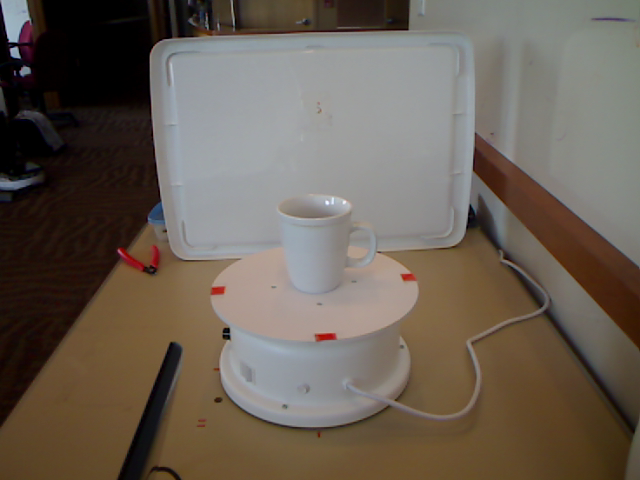
\includegraphics[scale=0.24]{img/base_rgbd/scene.png}
        \caption{Frame RGB sin procesar}
    \end{subfigure}
    \quad
    \begin{subfigure}[b]{0.4\textwidth}
		\centering
        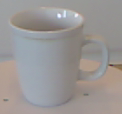
\includegraphics[width=0.8\textwidth]{img/base_rgbd/crop.png}
        \caption{Frame RGB recortado}
    \end{subfigure}
    \quad
    \begin{subfigure}[b]{0.4\textwidth}
		\centering
        
\includegraphics[width=\textwidth]{img/base_rgbd/maskcrop.png}
        \caption{Máscara sobre el frame RGB recortado que segmenta al objeto}
    \end{subfigure}
    \quad
    \begin{subfigure}[b]{0.4\textwidth}
		\centering
        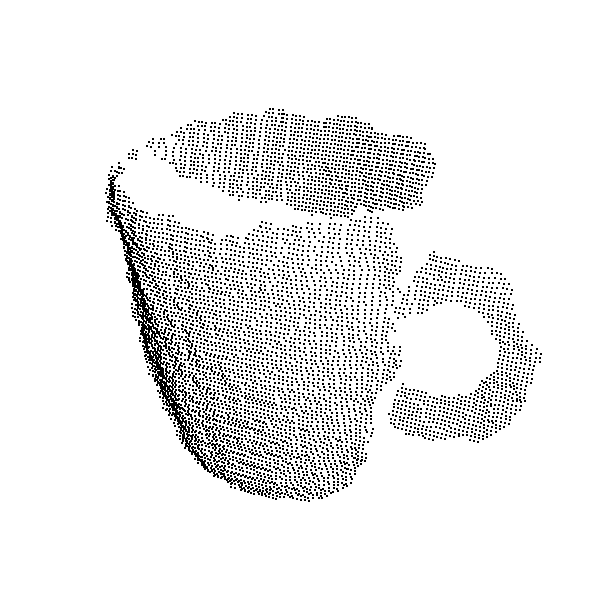
\includegraphics[width=\textwidth]{img/base_rgbd/cloud.png}
        \caption{Nube de puntos calculada con la información de profundidad}
    \end{subfigure}
    \caption{Datos que provee la base para cada frame de las escenas de los objetos. En este ejemplo, para una taza}
    \label{datos_objeto_base}
\end{figure}


Para tomar las escenas de los objetos se los filmó mientras giraban a velocidad constante en una base giratoria. La cámara RGB-D estaba ubicada a un metro de distancia y los videos se grabaron con la cámara montada a distintas alturas relativas a la base. Se filmó una secuencia por vuelta de cada objeto y para cada una de las alturas predefinidas. Cada uno de los frames de estas escenas viene acompañado de mucha información, como por ejemplo una imagen RGB más pequeña en donde está contenido el objeto, una máscara que permite segmentar al objeto del frame RGB, una nube de puntos del objeto segmentado para esa vista, etc. Esta información puede apreciarse en la Figura \ref{datos_objeto_base}.

\begin{figure}[t]
    \centering
    \begin{subfigure}[b]{0.4\textwidth}
		\centering
        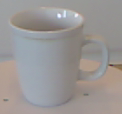
\includegraphics[width=0.8\textwidth]{img/base_rgbd/crop.png}
        \caption{Taza}
		\label{fig:taza}
    \end{subfigure}
    \quad
    \begin{subfigure}[b]{0.4\textwidth}
		\centering
        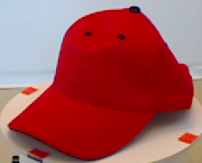
\includegraphics[width=\textwidth]{img/base_rgbd/gorra.png}
        \caption{Gorra}
		\label{fig:gorra}
    \end{subfigure}

    \quad
    \begin{subfigure}[b]{0.4\textwidth}
		\centering
        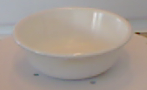
\includegraphics[width=\textwidth]{img/base_rgbd/bowl.png}
        \caption{Bowl}
		\label{fig:bowl}
    \end{subfigure}
	\quad
    \begin{subfigure}[b]{0.4\textwidth}
		\centering
        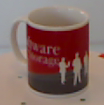
\includegraphics[width=0.8\textwidth]{img/base_rgbd/taza2.png}
        \caption{Taza 2}
		\label{fig:taza2}
    \end{subfigure}
	\quad
    \begin{subfigure}[b]{0.4\textwidth}
		\centering
        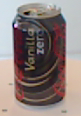
\includegraphics[scale=1.25]{img/base_rgbd/lata.png}
        \caption{Lata de gaseosa}
		\label{fig:lata}
    \end{subfigure}
	\quad
    \begin{subfigure}[b]{0.4\textwidth}
		\centering
        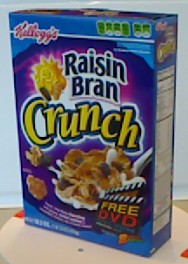
\includegraphics[scale=0.6]{img/base_rgbd/caja.png}
        \caption{Caja de cereales}
		\label{fig:caja}
    \end{subfigure}
    \caption{Muestra de objetos presentes en la base de datos.}
    \label{fig:ejemplo_objetos_base}
\end{figure}

Algunos de los objetos con los que cuenta la base de datos pueden verse en la Figura \ref{fig:ejemplo_objetos_base}. En esta selección vemos instancias objetos de distintas categorías, a excepción de las tazas de las figuras \ref{fig:taza} y \ref{fig:taza2} que son dos instancias distintas de la misma categoría.


\section{Escenas}
Sumado a las vistas de los objetos, la base cuenta con 8 secuencias de video RGB-D de escenas normales. Estas escenas cubren entornos cerrados comunes como oficinas, cocinas y sala de reuniones. Las escenas fueron grabadas sosteniendo el sensor RGB-D a la altura de los ojos de una persona mientras la persona que la sostenía caminaba alrededor de la escena. Los objetos que aparecen en la escena son capturados desde distintos ángulos y distancias, pudiendo estar o no ocluidos parcial o totalmente en algunos frames. De todos los objetos que componen la escena solo algunos se corresponden con objetos incluidos en la base de datos. Además, en cada escena se combinan distintas clases de objetos y distintas instancias de la misma clase, otorgando la posibilidad de verificar el comportamiento de algoritmos capaces de identificar instancias de objetos particulares o categorías de objetos según la clasificación de WordNet antes mencionada.

Estas escenas fueron anotadas de manera automática con información de ground truth sobre la ubicación de cada objeto en cada frame. En particular, la información de ground truth indica la posición de un bounding box que contiene a cada objeto en cada frame RGB.

\begin{figure}[t]
    \centering
    \begin{subfigure}[b]{0.4\textwidth}
		\centering
        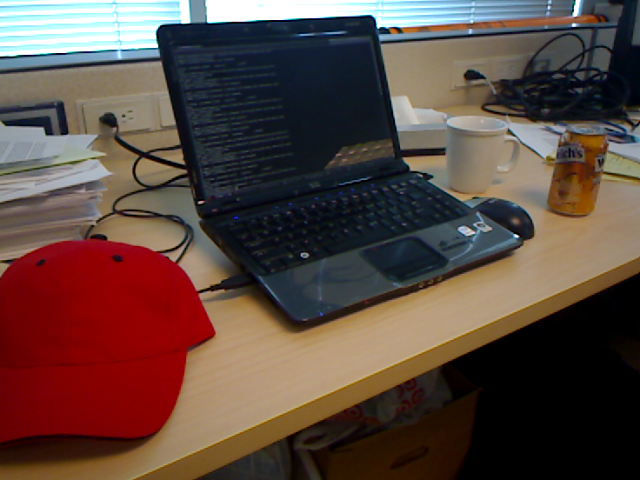
\includegraphics[width=\textwidth]{img/base_rgbd/desk_1.png}
        \caption{Escritorio 1 (desk\_1)}
		\label{fig:desk_1}
    \end{subfigure}
    \quad
    \begin{subfigure}[b]{0.4\textwidth}
		\centering
        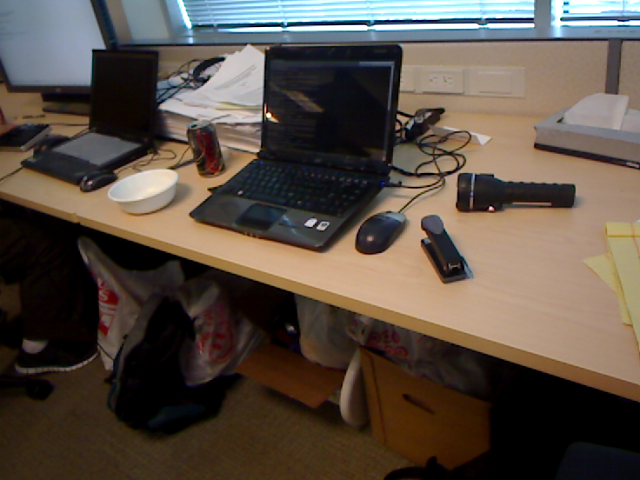
\includegraphics[width=\textwidth]{img/base_rgbd/desk_2.png}
        \caption{Escritorio 2 (desk\_2)}
		\label{fig:desk_2}
    \end{subfigure}

    \quad
    \begin{subfigure}[b]{0.4\textwidth}
		\centering
        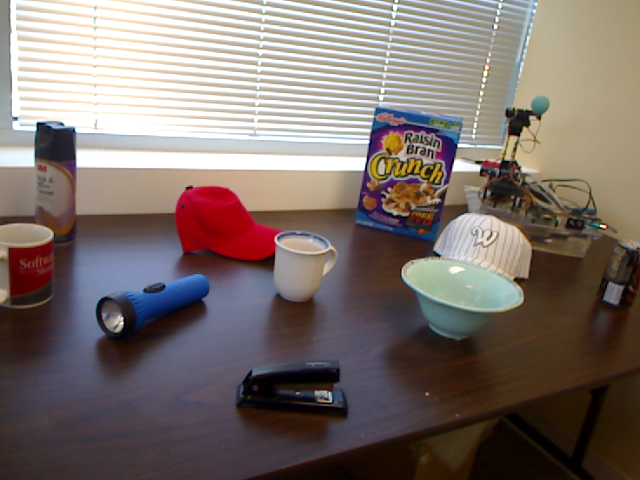
\includegraphics[width=\textwidth]{img/base_rgbd/table_1.png}
        \caption{Mesa 1 (table\_1)}
		\label{fig:table_1}
    \end{subfigure}
	\quad
    \begin{subfigure}[b]{0.4\textwidth}
		\centering
        \includegraphics[width=\textwidth]{img/base_rgbd/table_small_2.png}
        \caption{Mesa pequeña 2 (table\_small\_2)}
		\label{fig:table_small_2}
    \end{subfigure}

    \caption{Muestra de escenas presentes en la base de datos.}
    \label{fig:ejemplo_escenas_base}
\end{figure}

Algunas de las escenas con las que cuenta la base de datos pueden verse en la Figura \ref{fig:ejemplo_escenas_base}. En esta selección mostramos un frame de cada escena, aunque cada una está compuesta por varios frames. La escena llamada desk\_1 está compuesta por 98 frames, desk\_2 por 190, table por 125 y table\_small por 234.


\begin{figure}[t]
    \centering
    \begin{subfigure}[b]{0.3\textwidth}
        \includegraphics[width=\textwidth]{img/escena_rgbd/table_1_27.png}
    \end{subfigure}
    \quad
    \begin{subfigure}[b]{0.3\textwidth}
        \includegraphics[width=\textwidth]{img/escena_rgbd/table_1_34.png}
    \end{subfigure}
    \quad
    \begin{subfigure}[b]{0.3\textwidth}
        \includegraphics[width=\textwidth]{img/escena_rgbd/table_1_48.png}
    \end{subfigure}


    \begin{subfigure}[b]{0.3\textwidth}
        \includegraphics[width=\textwidth]{img/escena_rgbd/table_1_27_pcd.png}
    \end{subfigure}
    \quad
    \begin{subfigure}[b]{0.3\textwidth}
        \includegraphics[width=\textwidth]{img/escena_rgbd/table_1_34_pcd.png}
    \end{subfigure}
    \quad
    \begin{subfigure}[b]{0.3\textwidth}
        \includegraphics[width=\textwidth]{img/escena_rgbd/table_1_48_pcd.png}
    \end{subfigure}

    \caption{Frames de ejemplo tomados de la escena table\_1 de la base RGB-D. Cada columna tiene un frame RGB en la primer fila y su correspondiente nube de puntos en la segunda fila.}
    \label{fig:escena_rgbd_base}
\end{figure}

En la Figura \ref{fig:escena_rgbd_base} se muestran tres frames correspondientes a la escena table\_1. Para cada frame se muestra no solo su información RGB sino que además se adjunta una imagen de la nube de puntos correspondiente.


\section{Hardware}
Todas las secuencias de video de esta base de datos fueron capturadas utilizando un prototipo de cámara RGB-D fabricada por PrimeSense. Esta cámara graba simultáneamente imágenes RGB y de profundidad, cada una con una resolución de 640x480 píxeles y una frecuencia de 20 frames por segundo. Cada par de imágenes RGB y de profundidad provistos por la cámara están alineados y sincronizados, propiedades provistas por el driver de la cámara. Los puntos 3D en el espacio físico para cada píxel pueden obtenerse usando parámetros del sensor conocidos previamente.
